\documentclass[12pt,oneside,letterpaper]{book}
\usepackage[left=4cm,right=3cm,top=3cm,letterpaper,asymmetric]{geometry}
\usepackage[spanish, es-tabla]{babel}
\usepackage[utf8x]{inputenc}
\usepackage{titlesec} % Permite configurar los títulos de los capítulos, secciones, subsecciones, etc...
\usepackage{setspace}
\usepackage{graphicx}
\usepackage{xspace}
\usepackage{hyperref}
\usepackage[justification=centering]{caption}
\usepackage{amsmath}
\usepackage{amsthm}
\usepackage[table]{xcolor}
\usepackage{algorithm}
\usepackage{algpseudocode}
\usepackage{pifont}
\usepackage{listings}
%%%%%%%%%%%%%%%%%%%%%%%%%%%%%%%%%%%%%%%%%%%%%%%%%%%%%%%%%%%%%%%%%%%%%%%%
%%%%%%%% 					 Configurations						%%%%%%%%
%%%%%%%%%%%%%%%%%%%%%%%%%%%%%%%%%%%%%%%%%%%%%%%%%%%%%%%%%%%%%%%%%%%%%%%%
% Chapter title style
\titleformat{\chapter}[display]
	{\bfseries\Large}
	{\filleft\MakeUppercase{\chaptertitlename} \Huge\thechapter}
	{4ex}
	{\titlerule \vspace{2ex}\filright}

% Redefine command cleardoublepage like clearpage
\let\cleardoublepage\clearpage

% Paragraph
\setlength{\parindent}{1.25cm} % Indentacion de parrafos
\setlength{\parskip}{6pt plus 3pt minus 3pt} % Separacion entre parrafos
\linespread{1.5} % Separacion entre lineas

% Style commands
\newcommand{\gli}[2]{\item{\textbf{#1} #2}} % Elemento de Glosario
\newcommand{\eng}[1]{\textit{#1}\xspace}			% Termino en ingles
\newcommand{\abr}[1]{\textsc{#1}\xspace}           % Termino abreviado (gui, ...)

% Styling cell tables commands
\newcommand{\mycell}[1]{\cellcolor{gray!25}\color{blue}{#1}}

% Shortcut to write formal concepts in any enviroments
\newcommand{\formalconcept}[2]{$\langle #1,#2 \rangle$}
\newcommand{\formalconceptext}[4]{$\langle #1,#2 \rangle = \langle\{#3\},\{#4\}\rangle$}
\newcommand{\concept}[3]{$#1 = \langle\{#2\},\{#3\}\rangle$}

% Changing the bullet in itemize for a black circle
\renewcommand{\labelitemi}{$\bullet$}

\newcommand{\parallelbars}{\mathbin{\|}}

% Definitions styling
\theoremstyle{definition}
\newtheorem{definition}{Definición}[section]
\newtheorem{remark}{Observación}[section]

% New beta uppercase
\newcommand{\Beta}{\mathcal{B}}

 \floatname{algorithm}{Algoritmo}

\begin{document}
%%%%%%%%%%%%%%%%%%%%%%%%%%%%%%%%%%%%%%%%%%%%%%%%%%%%%%%%%%%%%%%%%%%%%%%%
%%%%%%%% 					Cover (Portada USM) 				%%%%%%%%
%%%%%%%%%%%%%%%%%%%%%%%%%%%%%%%%%%%%%%%%%%%%%%%%%%%%%%%%%%%%%%%%%%%%%%%%
\begin{titlepage}
\newgeometry{top=3cm}
\begin{centering}
{
\textbf{\Large UNIVERSIDAD TÉCNICA FEDERICO SANTA MARÍA}\\[0.3em]
\textbf{\small DEPARTAMENTO DE INFORMÁTICA}\\[0.85em]
\textbf{\small SANTIAGO -- CHILE}\\[2.4em]
}

\includegraphics[scale=0.295]{images/logo-utfsm} \\[4em]
\begin{spacing}{1.8}
\textbf{\Large \uppercase{``Distribución de Tópicos Emergentes en Conceptos Formales''}} \\[3.70em]
\end{spacing}
\textbf{\large \uppercase{Pablo Antonio Ortega Mesa}}\\[0.54em]
\textbf{\small MEMORIA DE TITULACIÓN PARA OPTAR AL TÍTULO DE INGENIERO CIVIL INFORMÁTICO} \\[1em]
\begin{tabular}{ccc} \small\bf
\small\bf PROFESOR GUÍA:          & & \small\bf \uppercase{Marcelo Mendoza} \\
\small\bf PROFESOR CORREFERENTE:  & & \small\bf \uppercase{Jose Luis Martí} \\
\end{tabular} \\[2.5em]
\textbf{\small JULIO -- 2015} \\
\end{centering}
\end{titlepage}
\restoregeometry



\begingroup
\titleformat{\chapter}[display]
  {\Large\scshape}
  {\thechapter}
  {-2em}
  {}
\titleformat{\section}
  {\Large\scshape}{\thesection}{2em}{}
%%%%%%%%%%%%%%%%%%%%%%%%%%%%%%%%%%%%%%%%%%%%%%%%%%%%%%%%%%%%%%%%%%%%%%%%
%%%%%%%% 						Agradecimientos 				%%%%%%%%
%%%%%%%%%%%%%%%%%%%%%%%%%%%%%%%%%%%%%%%%%%%%%%%%%%%%%%%%%%%%%%%%%%%%%%%%
\section*{Agradecimientos}
\thispagestyle{empty}
Deseo agradecer en primer lugar a mi familia por haber creído en mi y haberme brindado todo el apoyo incondicional para continuar. El camino no fue fácil, pero siempre estuvieron ahí para felicitarme en mis logros y darme ánimos en mis derrotas. Gracias a ellos es donde estoy.

Agradezco a los profesores. Especialmente, quiero agradecer al profesor Marcelo Mendoza, que más que mi profesor guía en este largo trabajo, ha sido un modelo a seguir en el ámbito de la investigación y docencia. Además quiero agradecer al profesor Jose Luis Martí, quién con su gran voluntad y comprensión me facilitaron el camino para seguir adelante.

Gracias a mis compañeros de Universidad, el apoyo recibido me ha servido para pasar los momentos más duros y gracias por los momentos especiales vividos. En especial a Paola Yunis, Matias Henriquez y Luis Villena quienes mas que compañeros de Universidad, se han convertido en grandes amigos. Además Quiero agradecer a todos aquellos que comenzaron siendo alumnos en mis ayudantías, pero que hoy se han vuelto compañeros y amigos.

También he de dar un agradecimiento especial a Víctor Codocedo, quién sin sus conocimientos y paciencia, no hubiese sido posible realizar este trabajo.

Finalmente, quiero agradecer a mi novia, mi compañera, Valeska Valenzuela, quién sin su gran ayuda y apoyo incondicional, todo este proceso no hubiese sido posible. Al fin termina esta travesía larga y compleja, tú has sido testigo de cuán difícil ha sido el proceso, pero también sabes que ahora estaremos libres para forjar nuestro propio destino.

Gracias.


\clearpage

%%%%%%%%%%%%%%%%%%%%%%%%%%%%%%%%%%%%%%%%%%%%%%%%%%%%%%%%%%%%%%%%%%%%%%%%
%%%%%%%% 							Resumen			 			%%%%%%%%
%%%%%%%%%%%%%%%%%%%%%%%%%%%%%%%%%%%%%%%%%%%%%%%%%%%%%%%%%%%%%%%%%%%%%%%%
\section*{Resumen}
\thispagestyle{empty}
En la actualidad, el uso masivo de Internet y sus redes de comunicación han provocado un crecimiento explosivo en la información que se puede encontrar en línea. Millones de páginas proveen a usuarios con innumerables contenidos, donde cada cuál contiene múltiples tópicos, de los cuales pueden llegar a ser relevantes o no para los usuarios. Es por esto que realizar una búsqueda por un tema muy específico, puede llevar demandar un gran consumo de tiempo y recursos.Particularmente para la comunidad científica es un gran problema encontrar los documentos científicos indicados que sean relevantes al trabajo que se esta realizando.

En este trabajo se propone generar una clusterización jerárquica suave mediante la técnica \abr{FCA} y observar la distribución de tópicos emergentes, que son generados utilizando la técnica \abr{LDA} que existen en cada clúster. De esta forma se permitirá al científico navegar en un grafo conceptual de acuerdo a los títulos de los documentos científicos presentes en la colección que está disponible mediante \abr{DBLP}.
\clearpage

%%%%%%%%%%%%%%%%%%%%%%%%%%%%%%%%%%%%%%%%%%%%%%%%%%%%%%%%%%%%%%%%%%%%%%%%
%%%%%%%% 							Abstract			 		%%%%%%%%
%%%%%%%%%%%%%%%%%%%%%%%%%%%%%%%%%%%%%%%%%%%%%%%%%%%%%%%%%%%%%%%%%%%%%%%%
\section*{Abstract}
\thispagestyle{empty}
Today, the massive use of Internet and communication networks have led to an explosive growth in the information that can be found online. Million pages provide users with many contents, where each contains multiple topics, which can become relevant or not for users. That is why searching for a very specific topic, may lead to demand a time-consuming. For the scientific community is a big problem find out the relevant scientific paper to the work that is being done.

This work aims to generate a smooth hierarchical clustering by \abr{FCA} and observe the distribution of emerging topics generated using  \abr{LDA} that exist in each cluster. Thus the scientist will be allowed to browse on a conceptual graph according to the titles of scientific papers in the collection is available through \abr{DBLP}
\clearpage

%%%%%%%%%%%%%%%%%%%%%%%%%%%%%%%%%%%%%%%%%%%%%%%%%%%%%%%%%%%%%%%%%%%%%%%%
%%%%%%%% 							Glosario			 		%%%%%%%%
%%%%%%%%%%%%%%%%%%%%%%%%%%%%%%%%%%%%%%%%%%%%%%%%%%%%%%%%%%%%%%%%%%%%%%%%
\section*{Glosario}
\thispagestyle{empty}
\begin{itemize}
	\gli{Tokenización}{Es la división de un texto en palabras, frases, símbolos u otros elementos significativos en estructuras llamadas \eng{tokens}.}
	\gli{Token}{Unidades mínimas con significado para un lenguaje en particular, generalmente palabras reservadas o nombres de variable.}
	\gli{Clustering}{Agrupamiento de sistemas independientes relacionados entre si.}
	\gli{XML}{\eng{eXtensible Markup Language}.}
	\gli{GEXF}{\eng{Graph Exchange XML Format}.}
	\gli{CSV}{(\eng{Comma-Separated Value}) Es un tipo de archivo para la representación de datos tabulados por medio de la utlización de \eng{coma} o \eng{punto y coma}.}
	\gli{DBLP}{\eng{Digital Bibliography and Library Project}.}
	\gli{LDA}{\eng{Lattent dirichet Allocation}.}
	\gli{FCA}{\eng{Formal Concept Analysis}.}
	\gli{Top terms}{lista de términos relevantes para un tema.}
	\gli{TMT}{\eng{Stanford Topic Modeling Toolbox}.}
	\gli{Grafo}{Conjunto de objetos llamados vértices o nodos unidos por enlaces llamados aristas o arcos.}
\end{itemize}
\clearpage


\tableofcontents
\clearpage
% \listoffigures
% \clearpage
% \listoftables
% \clearpage


\endgroup
\setcounter{page}{1}
\pagenumbering{roman}
%%%%%%%%%%%%%%%%%%%%%%%%%%%%%%%%%%%%%%%%%%%%%%%%%%%%%%%%%%%%%%%%%%%%%%%%
%%%%%%%% 					Introducción 						%%%%%%%%
%%%%%%%%%%%%%%%%%%%%%%%%%%%%%%%%%%%%%%%%%%%%%%%%%%%%%%%%%%%%%%%%%%%%%%%%
\chapter{Introducción}
\pagenumbering{arabic}
En la actualidad, el uso masivo de Internet y sus redes de comunicación han provocado un crecimiento explosivo en la información que se puede encontrar en línea. Millones de páginas proveen a usuarios con innumerables contenidos, donde cada cuál contiene múltiples tópicos, de los cuales pueden llegar a ser relevantes o no para los usuarios. Es por esto que realizar una búsqueda por un tema muy específico, puede llevar demandar un gran consumo de tiempo y recursos.

Junto a lo anterior, cada vez es más fácil el acceso a esta información por parte de los usuarios. Prácticamente lo único que se requiere es una conexión a Internet para tener acceso a una cantidad inconmensurable de información. Esto produce que se vayan conformando comunidades de usuarios en torno a ciertos tópicos de información. Estas comunidades de usuarios en los últimos años han adquirido una vital importancia para muchas áreas. Por ejemplo, en el área de la publicidad es útil para segmentar el mercado a quién dirigir las campañas publicitarias y así saber a qué publico objetivo ofrecer los productos, así un sinfín de consecuencias pueden ser observadas de acuerdo a estas comunidades de usuarios.

Particularmente, una de estas comunidades de usuarios es la comunidad científica, la cual es conformada por todos aquellos que deseen obtener o contribuir información en formato de artículos científicos en torno a un área de investigación. Dentro de la información que maneja esta comunidad, se encuentran cientos de años de historia científica en donde se pueden apreciar grandes descubrimientos y propuestas de nuevas técnicas, teóricas, entre otras cosas. Los científicos, para poder desarrollar sus investigaciones, requieren consumir una cantidad importante de conocimiento entregado por estos artículos, por lo que, la comunidad científica tiene la necesidad de tener nuevas herramientas que le permitan explorar y navegar a través de grandes colecciones de documentos científicos.

Para lograr esto, organizaciones como JSTOR\footnote{\url{http://www.jstor.org/}} o DBLP\footnote{\url{http://dblp.uni-trier.de/db/}} mantienen en sus bases de datos grandes cantidades de publicaciones científicas, las cuales cubren cientos de años de investigación. El objetivo de estas organizaciones no es almacenar la documentación científica completa, mas bien, intentan mantener una enorme \emph{colección bibliográfica} de alta calidad.

En consecuencia, los científicos modernos tienen acceso a enormes librerías digitales en donde se enfrentan a millones de artículos relacionados con su campo de trabajo. Buscar dentro de estas librerías utilizando un buscador simple podría ser una forma muy deficiente de obtener los resultados esperados.

Efectivamente, la comunidad científica requiere interactuar con estas grandes colecciones de artículos de una forma mas estructurada: buscando artículos similares a un interés determinado y explorar la colección resultante en base a los tópicos que emergen de estos documentos.

Sin embargo, el principal problema es la generación de una estructura que permita indexar los tópicos contenidos en un documento con otros que tengan el mismo tipo de tópicos. Dicha tarea no es posible hacerlo manualmente en la mayoría de las colecciones modernas debido al tamaño y la tasa de crecimiento. Por lo que, para desarrollar las herramientas necesarias para explorar y navegar las grandes librerías científicas digitales, se requiere métodos automáticos que permitas organizar, administrar y entregar los contenidos de las mismas.

Es por esto que en este trabajo se intentará resolver las problemáticas planteadas: alta dimensionalidad de los datos debido al gran tamaño y rápido crecimiento de las colecciones de artículos científicos, descubrimiento de tópicos emergentes entre los documentos, clasificación y organización de estos tópicos y navegación a través de la clasificación resultante para poder dar al científico un punto de partida para que pueda buscar los artículos que son de su interés.


%%%%%%%%%%%%%%%%%%%%%%%%%%%%%%%%%%%%%%%%%%%%%%%%%%%%%%%%%%%%%%%%%%%%%%%%
%%%%%%%% 					Objetivos	 						%%%%%%%%
%%%%%%%%%%%%%%%%%%%%%%%%%%%%%%%%%%%%%%%%%%%%%%%%%%%%%%%%%%%%%%%%%%%%%%%%
\chapter{Objetivos}
\section{Objetivo General}
\label{sec:objetivo_general}
El objetivo principal de la memoria es la construcción de un grafo coloreado
basado en una agrupación jerárquica de documentos científicos y tópicos inferidos
estadísticamente que sea capaz de navegar y visualizar los grupos que son similares 
entre sí.

\section{Objetivos Específicos}
\label{sec:objetivos_especificos}
\begin{itemize}
	\item Generar una clusterización jerárquica de una base de datos científica.
	Los artículos indexados por DBLP, pueden ser observados como un conjunto de términos relevantes que lo constituyen. Al realizar una clusterización adecuada que permita generar un orden jerárquico de clústeres en base a estos términos relevantes, se estará agrupando los documentos en relación a los \eng{tokens} que lo forman.

	\item Inferir tópicos emergentes entre los documentos.
	Los documentos científicos pueden ser representado por una mezcla de tópicos, donde cada tópico corresponde a una distribución de palabras o términos. Aplicando técnicas de inferencia estadística, se puede inferir los tópicos que emergen de los documentos, así como también, se puede calcular la probabilidad que un término pertenezca a un tópico o bien, que probabilidad existe que este tópico represente un determinado documento.

	\item Construir una visualización que permita al usuario navegar a través de cada clúster y observar los objetos que lo componen.
	Hoy en día, existen herramientas muy poderosas en cuanto a la visualización de grandes tamaños de contenidos. Por otro lado, para fomentar la interactividad con el usuario, existen muchas librerías que permiten entregar la sensación de navegar dentro de una determinada estructura de información al usuario.
\end{itemize}

%%%%%%%%%%%%%%%%%%%%%%%%%%%%%%%%%%%%%%%%%%%%%%%%%%%%%%%%%%%%%%%%%%%%%%%%
%%%%%%%% 					Marco Teórico 						%%%%%%%%
%%%%%%%%%%%%%%%%%%%%%%%%%%%%%%%%%%%%%%%%%%%%%%%%%%%%%%%%%%%%%%%%%%%%%%%%
\chapter{Marco Teórico}
\section{\abr{DBLP}}
\label{sec:dblp}
\abr{DBLP} (\eng{Digital Bibliography and Library Project})~\cite{DBLPLey2002} es un sitio web que posee una gran cantidad de documentación bibliográfica de artículos relacionados con ciencias de la computación. El sitio está alojado en la Universidad de Trier, Alemania. Originalmente, en los años 80's, fue una base de datos que almacenó referencias relacionadas con programación lógica. Actualmente, DBLP lista más de un millón de artículos: Algunos de ellos pertenecientes a \abr{VLDB} (\eng{Very Large Database}, en inglés; una revista acerca de bases de datos con mucho contenido), artículos de la \abr{IEEE} y \abr{ACM}, así como también artículos científicos de distintas conferencias.

\section{FCA}
\label{sec:fca}
\subsection{¿Qué es \eng{Formal Concept Analysis}?}
\label{sub:que_es_formal_concept_analysis}
\abr{FCA} es un método de análisis de datos que ha adquirido una gran popularidad a través de varios dominios de conocimiento.  \abr{FCA} analiza la información la cual describe la relación entre un particular conjunto de objetos y atributos. Esta información (objetos y atributos) puede ser la representación de muchas áreas de las actividades de la vida moderna.

\abr{FCA} produce dos tipos de salidas. La primera es el \eng{Concept Lattice} (entramado de conceptos), el cual es una colección de conceptos formales (clústeres) los cuales están ordenados jerárquicamente por una relación de subconcepto – súper concepto. Los conceptos formales son clústeres particulares los cuales representan conceptos naturales humanos, tales como ``organismo vivo en el agua'',  ``automóvil con sistema de manejo en todas las ruedas'', ``número divisible por 3 y por 4'', etc.

La segunda salida de \abr{FCA} es una colección de ``implicaciones de los atributos''. Una implicación de los atributos describe una particular dependencia entre los clústeres que es válida en los datos de entrada, como por ejemplo ``cada número divisible por 3 y 4 es divisible por 6'', ``cada encuestado con edad sobre 60 está retirado'', etc.

En relación con el procesamiento conceptual de data y conocimiento, \abr{FCA} tiene una integración inherente en tres componentes:
\begin{itemize}
	\item Descubrimiento de conceptos en los datos.
	\item Descubrimiento de dependencia en los datos.
	\item Visualización de datos, conceptos, y dependencias con ciertas capacidades las cuales pueden estar presentes o no.
\end{itemize}

La integración de estos tres componentes, hace a \abr{FCA} una herramienta poderosa y es por esto que ha sido aplicada para encontrar la solución a problemas en distintas disciplinas. Los ejemplos de aplicación de \abr{FCA} que se pueden encontrar incluyen la organización jerárquica de resultados de búsquedas en la web dentro de conceptos basados en tópicos comunes; análisis de datos de expresión de genes; recuperación de información; análisis y entendimiento de código de software, depuración, minería de datos, y diseño en ingeniería de software; aplicaciones de Internet como análisis y organización de colecciones de documentos y correos electrónicos; taxonomías anotadas y muchos otros proyectos de análisis de datos descritos en la literatura. Incluso, \abr{FCA} fue aplicado en contra-terrorismo. Esto fue reportado por el artículo de ``\eng{The N.S.A.’s Math Problem}'' por la edición del 16 de Mayo del 2006 del \eng{New York Times}.

\subsection{Primer Ejemplo utilizando \abr{FCA}} % (fold)
\label{sub:primer_ejemplo}
Una tabla d atributos lógicos se puede representar por la tripleta $\langle X,Y,I \rangle$ donde $I$ es la relación binaria entre $X$ e $Y$. Los elementos de $X$ son llamados objetos y corresponden a las filas de la tabla. Por otro lado, los elementos de $Y$ son llamados atributos y corresponden a las columnas de la tabla.

Además, para $x \in X$ e $y \in Y$, $\langle x,y\rangle \in I$ indica que el objeto $x$ tiene el atributo $y$. Mientras que $\langle x,y \rangle \notin I$ indica que $x$ no tiene $y$.

\clearpage
Por ejemplo, la Tabla~\ref{tbl:table_logical_attributes} (izquierda) representa una tabla con atributos lógicos. La correspondiente tripleta $\langle X,Y,I \rangle$ está dada por $X = \{x_1,x_2,x_3, x_4\}$, $Y = \{y_1,y_2,y_3\}$ y se tiene que $\langle x_1,y_1 \rangle \in I$, $\langle x_2,y_3 \rangle \notin I$, etc.
\begin{table}[h!]
	\centering
	\begin{minipage}[b]{0.49\textwidth}
		\begin{tabular}{|c|cccc|}
			\hline
				  & $y_1$	 & $y_2$ 	& $y_3$	   & $\dots$ \\
			\hline
			$x_1$ & $\times$ & $\times$ & $\times$ & 		  \\
			$x_2$ & $\times$ & $\times$ & 		   & $\vdots$ \\
			$x_3$ & 		 & $\times$ & $\times$ & 		  \\
			$\vdots$ & 		 & $\dots$	& 		   & $\ddots$ \\
			\hline		 	
		\end{tabular}
	\end{minipage}
	\begin{minipage}[b]{0.49\textwidth}
		\begin{tabular}{|c|cccc|}
			\hline
					 & $y_1$ & $y_2$   	& $y_3$ & $\dots$	\\
			\hline
			$x_1$	 & $1$ 	 & $1$	 	& $0.7$ & 			\\
			$x_2$	 & $0.8$ & $0.6$ 	& $0.1$ & $\vdots$	\\
			$x_3$	 & $0$	 & $0.9$ 	& $0.9$ & 			\\
			$\vdots$ & 		 & $\dots$	& 		& $\ddots$ 	\\
			\hline		 	
		\end{tabular}
	\end{minipage}
	\caption{Tabla con atributos lógicos: binario a la derecha y \eng{fuzzy} a la izquierda}
	\label{tbl:table_logical_attributes}
\end{table}

La representación las tablas de atributos lógicos como tripletas es muy común en \abr{FCA} y se menciona solo ``tabla $\langle X,Y,I \rangle$'' en vez de ``tripleta $\langle X,Y,I \rangle$ representante de la tabla dada''. \abr{FCA} busca obtener dos salidas de esa tabla. La primera llamada \eng{Concept Lattice} es una colección parcialmente ordenada de clústeres particulares de objetos y atributos. La segunda salida consiste en formulas llamadas \eng{attribute implications}, las cuales describen las dependencias de atributos particulares que se cumplen en la la información proporcionada por la tabla.

Los clústeres, llamados \eng{Formal Concepts}, son pares $\langle A,B \rangle$ donde $A \subseteq X$ es un conjunto de objetos y $B \subseteq Y$ es un conjunto de atributos. Tal que $A$ es un conjunto de todos los objetos que tienen todos los atributos de $B$, y por otra parte, $B$ es el conjunto de todos los atributos que son comunes en todos los objetos de $A$. Por ejemplo, $\langle \{x_1, x_2\}, \{y_1, y_2\} \rangle$ y $\langle \{x_1, x_2, x_3\}, \{y_2\} \rangle$ son ejemplos de \eng{formal concepts} de la tabla~\ref{tbl:table_logical_attributes} izquierda (al menos la parte visible).

Un \eng{attribute implication} es una expresión $A \Rightarrow B$ con $A$ y $B$  como conjuntos de atributos. $A \Rightarrow B$ es verdadero en la tabla $\langle X,Y,I \rangle$ si cada objeto tiene todos los atributos de $A$ como también todos los atributos desde $B$. Por ejemplo, $\{y_3\} \Rightarrow \{y_2\}$ es verdadero en la Tabla~\ref{tbl:table_logical_attributes}, mientras que $\{y_1,y_2\} \Rightarrow \{y_3\}$ no lo es ($x_2$ sirve como contra ejemplo).

\subsection{Raíces Históricas y Desarrollo} % (fold)
\label{sub:ra_ces_historicas_y_desarrollo}
A pesar que existen previos intentos, es comúnmente aceptado que \abr{FCA} comenzó con el artículo de Wille~\cite{wille1982}. En el cual provee un cuidadoso desarrollo del fundamento matemático de la técnica, el cual fue útil luego para desarrollar el fundamento computacional como uno de las fuertes características de \abr{FCA}. Otra de sus características es la noción simple y robusta de ``concepto'' inspirado en un enfoque tradicional que los tratan como lógica tradicional. 

La introducción y las aplicaciones de \abr{FCA} se describen en el trabajo de Carpineto y Romano~\cite{carpineto2004}, los fundamentos matemáticos están cubiertos por Ganter~\cite{Ganter1997} y el estado del arte esta tratado en el trabajo de Ganter et. al.~\cite{Ganter2005}

\subsection{\eng{Concept Lattices}}
\label{sub:concept_lattices}
Esta sección introduce las nociones básicas y estructuras matemáticas asociadas de \eng{formal concept analysis}, entre donde podemos entronar los conceptos fundamentales como son \eng{formal context}, \eng{formal concept} y \eng{concept lattice}.

\subsubsection{Datos de Entrada}
\label{ssub:datos_de_entrada}
En una configuración básica, los datos de entrada de \abr{FCA} se encuentran en la forma de tabla (llamada \eng{cross-table}), la cual describe la relación entre los objetos (representados por las filas de la tabla) y atributos (representados por las columnas de la tabla). Un ejemplo se puede apreciar en la Tabla~\ref{tbl:cross_table}. La entrada $\times$ indica que el objeto tiene el correspondiente atributo.

\begin{table}[h!]
	\centering
	\begin{tabular}{|c|cccc|}
		\hline
		$I$		& $y_1$		& $y_2$ 	& $y_3$ 	& $y_4$ 	\\ \hline
		$x_1$	& $\times$	& $\times$	& $\times$ 	& $\times$ 	\\
		$x_2$	& $\times$	& 			& $\times$ 	& $\times$ 	\\
		$x_3$	& 			& $\times$	& $\times$ 	& $\times$ 	\\
		$x_4$	& 			& $\times$	& $\times$ 	& $\times$ 	\\
		$x_5$	& $\times$	& 			& 		 	& 		 	\\
		\hline
	\end{tabular}
	\caption{\eng{cross-table}}
	\label{tbl:cross_table}
\end{table}

\newpage
Por ejemplo, si los objetos que se modelaron son productos como automóviles y los atributos corresponden a características de dichos automóviles como es ``tiene sistema \abr{ABS}'', el símbolo $\times$ en la tabla indica que ese particular automóvil tiene \abr{ABS} (\eng{anti-block breaking system}). Por otra parte, si una entrada de la tabla está en blanco, indica que el objeto no tiene el atributo (un particular automóvil puede no tener sistema \abr{ABS}). Esto es, en la Tabla~\ref{tbl:cross_table}, el objeto $x_2$ tiene el atributo $y_1$ pero no tiene el atributo $y_2$.

Formalmente, una \eng{cross-table} es representada por lo que se llama un \eng{Formal Context}.

\theoremstyle{definition}
\begin{definition}{(\eng{formal context})}
Un \eng{formal context} is una tripleta $\langle X,Y,I \rangle$ donde $X$ e $Y$ son conjuntos no vacíos e $I$ es una relación binaria entre $X$ e $Y$. Es decir, $I \subseteq X \times Y$.
\end{definition}

Para un \eng{formal context}, los elementos $x$ de $X$ son llamados objetos y los elementos $y$ de $Y$ son los llamados atributos. $\langle x,y \rangle \in I$ indica que el objeto $x$ tiene el atributo $y$. Dada una \eng{cross-table} con $n$ filas y $m$ columnas, el contexto formal $\langle X,Y,I \rangle$ consiste en los conjuntos $X = \{x_1,\dots,x_n\}$, $Y = \{y_1,\dots,y_m\}$, y la relación $I$ definida por $\langle x_i,y_j \rangle \in I$ si y solo sí existe una entrada en la tabla correspondiente a la fila $i$ y columna $j$ que contiene $\times$. 

\subsubsection{Operadores de Formación de Conceptos}
\label{ssub:operadores_de_formacion_de_conceptos}
Cada \eng{formal concept} induce un par de operadores, llamados \eng{concept-forming operators} (operadores de formación de conceptos). 

\begin{definition}{(Operadores de formación de conceptos)}
Dado un \eng{formal context} $\langle X,Y,I \rangle$, los operadores $^{\uparrow}: 2^X \rightarrow 2^Y$ y $^{\downarrow}: 2^Y \rightarrow 2^X$ están definidos para cada $A \subseteq X$ y $B \subseteq Y$ por
\begin{eqnarray}
	A^{\uparrow} 	&=& \{y \in Y|\text{ para cada } x \in A: \langle x,y \rangle \in I\}, \nonumber \\
	B^{\downarrow} 	&=& \{x \in X|\text{ para cada } y \in B: \langle x,y \rangle \in I\}. \nonumber
\end{eqnarray}
\end{definition}

\begin{remark}[]
\begin{itemize}
	\item El operador $^{\uparrow}$ asigna subconjuntos de $Y$ a subconjuntos de $X$. $A^{\uparrow}$ es el conjunto de atributos que comparten todos los objetos de A.
	\item Por otro lado, el operador $^{\downarrow}$ asigna subconjuntos de $X$ a subconjuntos de $Y$. $B^{\downarrow}$ es el conjunto de todos los objetos que comparten todos los atributos de $B$.
	\item Para enfatizar $^{\uparrow}$ y $^{\downarrow}$ se induce a través de $\langle X,Y,I \rangle$, se usa $^{\uparrow_I}$ y $^{\downarrow_I}$
\end{itemize}
\end{remark}

Por ejemplo, para los operadores de formación de conceptos de la Tabla~\ref{tbl:cross_table} se tiene:
\begin{itemize}
 	\item $\{x_2\}^{\uparrow} = \{y_1, y_3, y_4\}, \{x_2,x_3\}^{\uparrow} = \{y_3, y_4\}$,
 	\item $\{x_1, x_4, x_5\}^{\uparrow} = \emptyset$,
 	\item $X^{\uparrow} = \emptyset, \emptyset^{\uparrow} = Y$,
 	\item $\{y_1\}^{\downarrow} = \{x_1,x_2,x_5\}, \{y_1,y_2\}^{\downarrow} = \{x_1\}$,
 	\item $\{y_2,y_3\}^{\downarrow} = \{x_1,x_3,x_4\}, \{y_2,y_3,y_4\}^{\downarrow} = \{x_1,x_3,x_4\}$
 	\item $\emptyset^\downarrow = X, Y^\downarrow = \{x_1\}$.
 \end{itemize}

 \subsubsection{\eng{Formal Concepts} y \eng{Concept Lattice}}
 \label{ssub:formal_concept_concept_lattice}
 La noción de ``conceptos formales'' es fundamental en \abr{FCA}. Un concepto formal es un particular clúster de la \eng{cross-table}, definido por medio de los atributos que comparten.

 \begin{definition}{(\eng{Formal Concept})}
 Un \eng{formal concept} en la tripleta $\langle X,Y,I \rangle$ es un par $\langle A,B \rangle$ de $A \subseteq X$ y $B \subseteq Y$ tal que $A^\uparrow = B$ y $B^\downarrow = A$.
 \end{definition}

 Dado un concepto formal $\langle A,B \rangle$ en $\langle X,Y,I \rangle$, $A$ y $B$ son llamados \eng{extent} e \eng{intent} de $\langle A,B \rangle$ respectivamente. Una descripción verbal de un concepto formal se presenta a continuación: ``$\langle A,B \rangle$ es un concepto formal si y solo si $A$ contiene sólo los objetos que comparten todos los atributos de $B$ y, por otra parte, $B$ contiene solo los atributos que son compartidos por todos los objetos de $A$''. Matemáticamente, $\langle A,B \rangle$ es un concepto formal si y solo si $\langle A,B \rangle$ es un \eng{fixpoint} del par $\langle ^\uparrow, ^\downarrow\rangle$ de los operadores formadores de conceptos.

 Por ejemplo, en la Tabla~\ref{tbl:cross_table_highlighted}, 
\begin{table}[h!]
	\centering
	\begin{tabular}{|c|cccc|}
		\hline
		$I$		& $y_1$		& $y_2$ 	& $y_3$ 				& $y_4$ 				\\ \hline
		$x_1$	& $\times$	& $\times$	& \mycell{$\times$} 	& \mycell{$\times$} 	\\
		$x_2$	& $\times$	& 			& \mycell{$\times$} 	& \mycell{$\times$} 	\\
		$x_3$	& 			& $\times$	& \mycell{$\times$} 	& \mycell{$\times$} 	\\
		$x_4$	& 			& $\times$	& \mycell{$\times$} 	& \mycell{$\times$} 	\\
		$x_5$	& $\times$	& 			& 		 				& 		 				\\
		\hline
	\end{tabular}
	\caption{\eng{cross-table} resaltando a concepto $\langle A_1, B_1 \rangle$}
	\label{tbl:cross_table_highlighted}
\end{table}

se puede ver que el rectángulo resaltado representa el concepto formal
 \begin{equation*}
 	\langle A_1,B_1 \rangle = \langle\{x_1,x_2,x_3,x_4\}, \{y_3,y_4\}\rangle
 \end{equation*}

 debido a 
 \begin{equation*}
 	\{x_1,x_2,x_3,x_4\}^\uparrow = \{y_3,y_4\}\text{ y }\{y_3,y_4\}^\downarrow = \{x_1,x_2,x_3,x_4\}.
 \end{equation*}

Pero hay otros conceptos formales. Tres de ellos están representados por los siguientes rectángulos resaltados:

\begin{table}[h!]
	\centering
	\begin{tabular}{|c|cccc|}
		\hline
		$I$		& $y_1$				& $y_2$ 			& $y_3$ 				& $y_4$ 				\\ \hline
		$x_1$	& $\times$			& \mycell{$\times$}	& \mycell{$\times$} 	& \mycell{$\times$} 	\\
		$x_2$	& $\times$			& 					& $\times$				& $\times$				\\
		$x_3$	& 					& \mycell{$\times$}	& \mycell{$\times$} 	& \mycell{$\times$} 	\\
		$x_4$	& 					& \mycell{$\times$}	& \mycell{$\times$} 	& \mycell{$\times$} 	\\
		$x_5$	& $\times$			& 					& 		 				& 		 				\\
		\hline
	\end{tabular}
	\quad
	\begin{tabular}{|c|cccc|}
		\hline
		$I$		& $y_1$				& $y_2$ 			& $y_3$ 				& $y_4$ 				\\ \hline
		$x_1$	& \mycell{$\times$}	& $\times$			& \mycell{$\times$} 	& \mycell{$\times$} 	\\
		$x_2$	& \mycell{$\times$}	& 					& \mycell{$\times$} 	& \mycell{$\times$} 	\\
		$x_3$	& 					& $\times$			& $\times$ 				& $\times$ 				\\
		$x_4$	& 					& $\times$			& $\times$ 				& $\times$ 				\\
		$x_5$	& $\times$			& 					& 		 				& 		 				\\
		\hline
	\end{tabular}
	\quad
	\begin{tabular}{|c|cccc|}
		\hline
		$I$		& $y_1$				& $y_2$ 			& $y_3$ 				& $y_4$ 				\\ \hline
		$x_1$	& \mycell{$\times$}	& $\times$			& $\times$ 				& $\times$ 				\\
		$x_2$	& \mycell{$\times$}	& 					& $\times$ 				& $\times$ 				\\
		$x_3$	& 					& $\times$			& $\times$ 				& $\times$ 				\\
		$x_4$	& 					& $\times$			& $\times$ 				& $\times$ 				\\
		$x_5$	& \mycell{$\times$}	& 					& 		 				& 		 				\\
		\hline
	\end{tabular}
	\label{tbl:cross_table_highlighted2}
\end{table}

Donde, $\langle A_2,B_2 \rangle = \langle\{x_1,x_3,x_4\}, \{y_2,y_3,y_4\}\rangle$, $\langle A_3,B_3 \rangle = \langle \{x_1,x_2\},\{y_1,y_3,y_4\} \rangle$, y $\langle A_4,B_4 \rangle = \langle \{x_1,x_2,x_5\},\{y_1\} \rangle$.

La noción de \eng{formal concept} puede ser entendida como una simple matematización de la bien conocida noción de ``concepto'' que se basa en la lógica de \eng{Port-Royal}. De acuerdo a \eng{Port-Royal}, un concepto está determinado por una colección de objetos (\eng{extent}) y una colección de atributos (\eng{intent}) que comparten estos objetos. Además, los conceptos están ordenados naturalmente usando una relación de subconcepto-súperconcepto. Esta relación radica en la relación de inclusión sobre objetos y atributos. Formalmente, la relación subconcepto-súperconcepto se define como sigue. 

\begin{definition}{relación subconcepto-súperconcepto}
Para los conceptos dados por $\langle A_1,B_1 \rangle$ y $\langle A_2, B_2 \rangle$ de la tripleta $\langle X,Y,I \rangle$, se dice que $\langle A_1,B_1 \rangle \le \langle A_2,B_2 \rangle$ iff $A_1 \subseteq A_2$ (iff $B_2 \subseteq B_1$).
\end{definition}
\begin{remark}[]
	\begin{itemize}
		\item[--] $\le$ representa el ordenamiento entre subconcepto-súperconcepto.
		\item[--] $\langle A_1,B_1 \rangle \le \langle A_2,B_2 \rangle$ significa que $\langle A_1,B_1 \rangle$ es más específico que $\langle A_2,B_2 \rangle$. ($\langle A_2,B_2 \rangle$ es más general).
		\item[--] $\le$ captura la idea detrás de $\text{PERRO } \le \text{MAMÍFERO}$ (el concepto de perro es más específico que el concepto de mamífero). 
	\end{itemize}
\end{remark}

Por ejemplo, si consideramos los conceptos de la Tabla~\ref{tbl:cross_table}: \\ \formalconceptext{A_1}{B_1}{x_1,x_2,x_3,x_4}{y_3,y_4}, \formalconceptext{A_2}{B_2}{x_1,x_3,x_4}{y_2,y_3,y_4}, \formalconceptext{A_3}{B_3}{x_1,x_2}{y_1,y_3,y_4}, \formalconceptext{A_4}{B_4}{x_1,x_2,x_5}{y_1}. Luego \formalconcept{A_3}{B_3} $\le$ \formalconcept{A_1}{B_1}, \formalconcept{A_3}{B_3} $\le$ \formalconcept{A_2}{B_2}, \formalconcept{A_3}{B_3} $\le$ \formalconcept{A_4}{B_4}, \formalconcept{A_2}{B_2} $\le$ \formalconcept{A_1}{B_1}, \formalconcept{A_1}{B_1} $\parallelbars$ \formalconcept{A_4}{B_4} (incomparable), \formalconcept{A_2}{B_2} $\parallelbars$ \formalconcept{A_4}{B_4}.

La colección de todos los conceptos formales dado un contexto formal, se denomina \eng{concept lattice}, el cual es otra noción fundamental en \abr{FCA}.

\begin{definition}{(\eng{concept lattice})}
	Se denota por $\Beta(X,Y,I)$ a la colección de todos los \eng{formal concepts} de $\langle X,Y,I \rangle$, es decir
\begin{equation*}
	\Beta(X,Y,I) = \{\langle A,B\rangle \in 2^X\times2^Y | A^\uparrow = B, B^\downarrow = A\}.
\end{equation*}
\end{definition}

$\Beta(X,Y,I)$ provista con el ordenamiento de subconcepto-súperconcepto $\le$ se denomina \eng{concept lattice} de $\langle X,Y,I \rangle$.

\begin{itemize}
	\item $\Beta(X,Y,I)$ representa todos (potencialmente interesantes) clústeres que están ``escondidos'' en la data de $\langle X,Y,I \rangle$.
	\item Se puede entender que $\langle \Beta(X,Y,I),\le \rangle$ es un \eng{concept lattice}.
\end{itemize}

También se denota como
\begin{equation*}
	\text{Ext}(X,Y,I) = \{A \in 2^X | \langle A,B \rangle \in \Beta(X,Y,I) \text{ para algún }B \} \text{ (\eng{extent} de los conceptos)}
\end{equation*}
\begin{equation*}
	\text{Int}(X,Y,I) = \{A \in 2^Y | \langle A,B \rangle \in \Beta(X,Y,I) \text{ para algún }A \} \text{ (\eng{intent} de los conceptos)}.
\end{equation*}

Por ejemplo, si se considera la siguiente \eng{cross-table} ~\cite{Ganter1997}

\begin{table}[h!]
	\centering
	\begin{tabular}{|r|c||c|c|c|c|c|c|c|c|c|}
		\hline
		\multicolumn{2}{|c||}{}	& 	$a$ 		& 	$b$ 		& 	$c$ 		& 	$d$ 	 & 	$e$ 	 & 	$f$ 	 & 	$g$ 	 & 	$h$		 & 	$i$		 \\ \hline 
		\hline
		sanguijuela 			& 1 & 	$\times$ 	& 	$\times$ 	& 		 		& 		 	 & 		 	 & 		 	 & 	$\times$ & 			 & 			 \\ \hline
		brema (pez) 			& 2 & 	$\times$ 	& 	$\times$ 	& 		 		& 		 	 & 		 	 & 		 	 & 	$\times$ & 	$\times$ & 			 \\ \hline
		rana 					& 3 & 	$\times$ 	& 	$\times$ 	& 	$\times$ 	& 		 	 & 		 	 & 		 	 & 	$\times$ & 	$\times$ & 			 \\ \hline
		perro  					& 4 & 	$\times$ 	& 	        	& 	$\times$ 	& 		 	 & 		 	 & 		 	 & 	$\times$ & 	$\times$ & 	$\times$ \\ \hline
		pico de malezas			& 5 & 	$\times$ 	& 	$\times$ 	& 		 		& 	$\times$ & 		 	 & 	$\times$ & 		 	 & 			 & 			 \\ \hline
		caña 	 				& 6 & 	$\times$ 	& 	$\times$ 	& 	$\times$ 	& 	$\times$ & 		 	 & 	$\times$ & 		 	 & 			 & 			 \\ \hline
		haba 					& 7 & 	$\times$ 	& 	 			& 	$\times$ 	& 	$\times$ & 	$\times$ & 		 	 & 		 	 & 			 & 			 \\ \hline
		maíz	 				& 8 & 	$\times$ 	& 			 	& 	$\times$ 	& 	$\times$ & 		 	 & 	$\times$ & 		 	 & 			 & 			 \\ \hline
	\end{tabular}
	\caption{$a$: necesita agua para vivir; $b$: vive en el agua; $c$: vive en tierra; $d$: necesita clorofila para producir comida, $e$: dos semillas; $f$: una semilla; $g$: puede moverse; $h$: tiene extremidades; $i$: amamanta a sus crías.}
	\label{tbl:concept_lattice_full_example}
\end{table}

El correspondiente \eng{formal context} $\langle X,Y,I \rangle$ contiene los siguientes conceptos formales:

\concept{C_0}{1,2,3,4,5,6,7,8}{a}, \concept{C_1}{1,2,3,4}{a,g}, \concept{C_2}{2,3,4}{a,g,h}, \concept{C_3}{5,6,7,8}{a,d}, \concept{C_4}{5,6,8}{a,d,f}, \concept{C_5}{3,4,6,7,8}{a,c}, \concept{C_6}{3,4}{a,c,g,h}, \concept{C_7}{4}{a,c,g,h,i}, \concept{C_8}{6,7,8}{a,c,d}, \concept{C_9}{6,8}{a,c,d,f}, \concept{C_{10}}{7}{a,c,d,e}, \concept{C_{11}}{2,3}{a,b,g,h}, \concept{C_{12}}{1,2,3}{a,b,g}, \concept{C_{13}}{2,3}{a,b,g,h}, \concept{C_{14}}{5,6}{a,b,d,f}, \concept{C_{15}}{3,6}{a,b,c}, \concept{C_{16}}{3}{a,b,c,g,h}, \concept{C_{17}}{6}{a,b,c,d,f}, \concept{C_{18}}{}{a,b,c,d,e,f,g,h,i}.

El correspondiente \eng{concept lattice} $\Beta(X,Y,I)$ se aprecia en la Figura~\ref{fig:concept_lattice_full_example}

\begin{figure}[h!]
	\centering
	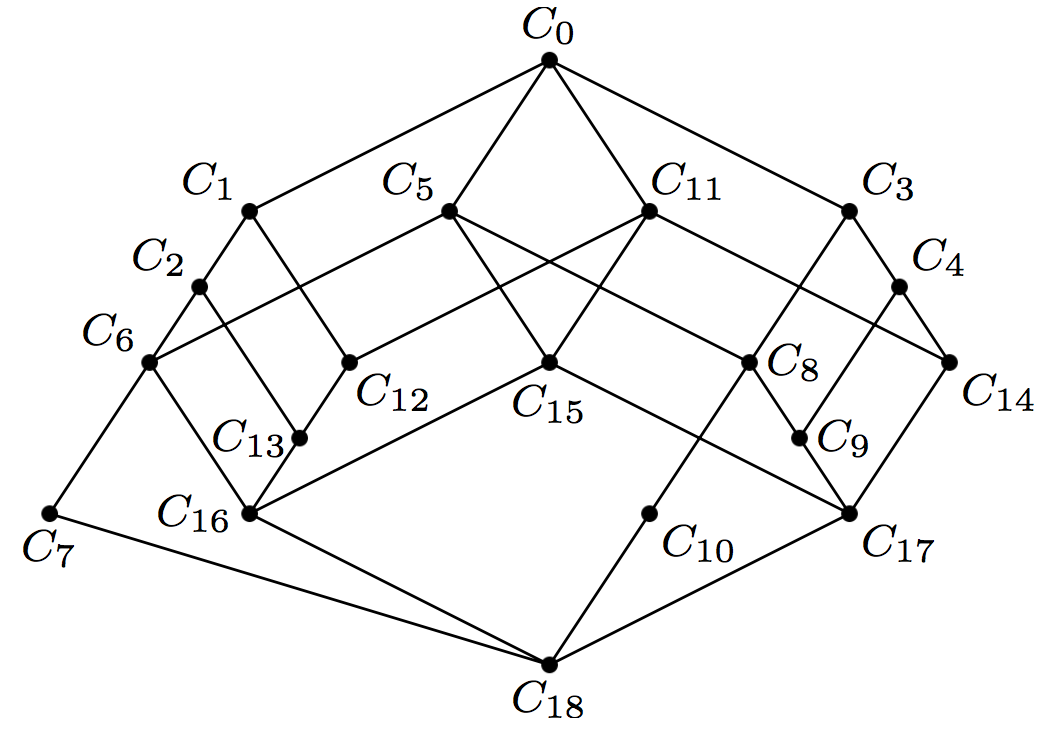
\includegraphics[width=0.90\textwidth]{images/conceptlattice.png}
	\caption{\eng{Concept Lattice} correspondiente a la información de la Tabla~\ref{tbl:concept_lattice_full_example}}
	\label{fig:concept_lattice_full_example}
\end{figure} 


\newpage


 \begin{definition}{(\eng{Support})}
 El \eng{support} \cite{CodocedoTA11} de un concepto formal dado por $\langle A,B \rangle$, donde $A \subseteq X$ y $B \subseteq Y$ está definido por:
 \begin{equation*}
	\text{\emph{supp}}(\langle A,B \rangle) = \frac{|A|}{|X|}
\end{equation*}
 \end{definition}

 \begin{definition}{(\eng{Frequent Concept})}
 Dado un umbral $\text{\eng{minsupp}} \in [0,1]$, entonces el concepto $\langle A,B \rangle$ es llamado \eng{Frequent Concept} si y sólo si $\text{\emph{supp}}(\langle A,B \rangle) \ge \text{\emph{minsupp}}$.
 \end{definition}

 \begin{definition}{(\eng{Iceberg Lattice})}
 Un \textbf{\eng{Iceberg Lattice}} es el conjunto de todos los \eng{Frequent Concepts} dado un \eng{minsupp}.
 \end{definition}

\section{Topic Models}
\label{sec:topic_models}
Los algoritmos de \eng{Topic Modeling} \cite{TopicModels2009} son usados para descubrir un conjunto de ``{tópicos}'' dentro de una gran colección de documentos, donde un {\bf tópico} es una distribución de términos los cuales están relacionados a través de un único tema. \eng{Topic Models} proveen una legible representación de baja dimensionalidad de los documentos \cite{Chang2009}. Estos algoritmos han sido usados para tareas como exploración de corpus, clasificación de documentos y recuperación de información.

El modelo mas simple de \eng{Topic Modeling} es \eng{Latent Dirichlet Allocation} \cite{BleiLDA2003}. En donde se asume que existen $K$ tópicos: $\boldsymbol\beta = \beta_{1:K}$, donde cada uno es una distribución de un vocabulario fijo. El proceso generativo de \emph{LDA} es como se describe a continuación. Por cada documento $w_j$ en la colección,

\begin{enumerate}
	\item Calcular las proporciones del tópico $\theta_j \sim \text{Dirichlet}(\alpha)$
	\item Por cada palabra $n$,
	\begin{enumerate}
		\item Calcular la asignación del tópico $z_{jn} \sim \text{Mult}(\theta_j)$.
		\item Calcular $w_{jn} \sim \text{Mult}(\beta_{z_{jn}})$
	\end{enumerate}
\end{enumerate}

Este proceso revela como se asume que las palabras de cada documento provienen de una mezcla de tópicos: las proporciones del tópico son por cada documento específico, pero el conjunto de tópicos es compartido por la colección.

\begin{figure}[h!]
	\centering
	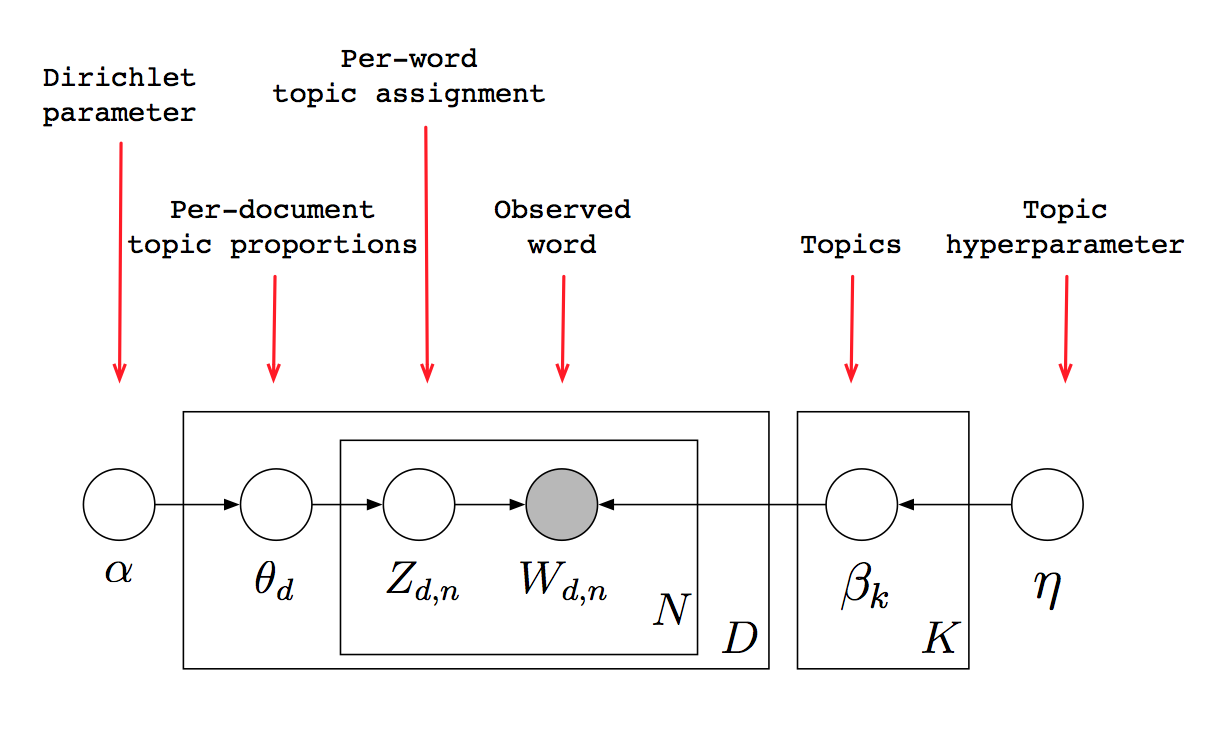
\includegraphics[width=0.95\textwidth]{images/lda.png}
	\caption{Representación gráfica del modelo \eng{LDA}}
	\label{fig:lda}
\end{figure}   

El modelo representado en la Figura~\ref{fig:lda} muestra como es posible generar un documento utilizando una mezcla de temas. El número de tópicos esta dado por la distribución finita $K$. Estos temas están compuestos por una distribución de palabras $\beta_k$, pertenecientes a un vocabulario en específico. La proporción de temas para un documento $d$, esta dada representada por $\theta_d$. $Z_d$ corresponde a los temas asignados al documento $d$. Luego $Z_{d,n}$ corresponde al tema asignado por la palabra $n$ en el documento $d$. Finalmente, la palabra observada para el documento $d$ es $w_d$, donde $w_{d,n}$ es la palabra $n$ en el documento $d$, que corresponde a una palabra de un vocabulario fijo.


%%%%%%%%%%%%%%%%%%%%%%%%%%%%%%%%%%%%%%%%%%%%%%%%%%%%%%%%%%%%%%%%%%%%%%%%
%%%%%%%% 				Descripción de Problemas 				%%%%%%%%
%%%%%%%%%%%%%%%%%%%%%%%%%%%%%%%%%%%%%%%%%%%%%%%%%%%%%%%%%%%%%%%%%%%%%%%%
\chapter{Descripción de Problemas}
\section{Base de Datos Científicas}
\label{sec:base_de_datos_cientificas}

% La comunidad científica consume grandes cantidades de información a través de diferentes fuentes, en donde podemos encontrar artículos de revistas, libros, tesis, bases de datos, conferencias y colaboraciones entre muchas otras. Particularmente, los artículos de revistas son la principal fuente de información para científicos. Por ejemplo, los ``Físicos'' leen un promedio de 204 artículos por año, mientras que los ``Químicos'' leen aproximadamente 276 artículos por año. Además, los científicos y médicos leen tres veces mas artículos de revistas que los profesionales de áreas legales, administración y ventas. Para encontrar estos artículos, los científicos buscan a través de revistas o buscan en base de datos bibliográficos. Por ejemplo, \eng{PubMed}\footnote{\url{http://www.ncbi.nlm.nih.gov/pubmed}} (\eng{National Library of Medicine}) tiene entre $500.000$ y $1.000.000$ búsquedas cada día.  
Una importante actividad de la comunidad científica es mantenerse al tanto de las investigaciones actuales dentro
del área donde trabajan. Los científicos utilizan muchas formas de comunicación, herramientas y servicios para encontrar artículos relevantes ~\cite{hoggan2002, tenopir2001}.

Una biblioteca, es una colección de registros del conocimiento humano, la cual es la mayor fuente de información para científicos. Los bibliotecarios sirven como mediadores entre los humanos y la colección bibliográfica en orden de maximizar la utilización de registros para el beneficio de la sociedad ~\cite{marsterson1986}.

La organización, el proceso y la funcionalidad de una biblioteca ha ido cambiando dramáticamente con la introducción de la tecnología, especialmente con la Web ~\cite{saunders1993}. Estos cambios han tenido un gran impacto en las formas que los científicos realizan sus investigaciones.

La Web provee un nuevo medio para almacenar, presentar, reunir, compartir, procesar y utilizar la información. Lleva a una nueva era de la información. Ahí hay una tremenda cantidad de material \eng{online} como periódicos, películas, música, revistas, y muchos otros productos y servicios. Conceptualmente, la Web puede ser observada como una gigante biblioteca virtual que permite búsquedas ~\cite{saunders1993}. Para realizar un uso efectivo de la Web para la comunidad científica produce un gran desafío.

Los científicos encaran muchos desafíos usando recursos basados en la Web para encontrar estos artículos, como son por ejemplo: sobrecarga de información, desinformación, pagos, navegación pobremente diseñada y herramientas de navegación y recuperación ~\cite{hoggan2002}. Existe una necesidad urgente de nuevos sistemas de información que soporten actividades de investigación académica y jueguen el rol de los tradicionales bibliotecarios.

Los sistemas de recuperación de información basados en la Web (\abr{WIRSS} por sus siglas en inglés) ayudan a las actividades básicas de científicos, como son recuperación, exploración, organización y utilización de la información en la Web ~\cite{yao2003web,yao2002information}. El objetivo de los \abr{WIRSS} para científicos es construir nuevas y mas eficientes herramientas de investigación para que la misma comunidad tome la ventaja de utilizar la Web. Con estas herramientas, la Web para la comunidad científica puede ser vista como una grande y personalizada base de conocimiento.

Una vez identificada las necesidades de un \abr{WIRSS}, es tentador el paso siguiente, crear nuevas teorías y construir nuevos sistemas. Sin embargo, el gran número de sistemas implementados que existen, comparados con la pequeña cantidad que en la práctica se ocupan sugiere que esta no podría ser la mejor opción. Es por esta razón que es útil pensar en un nuevo enfoque, como es el caso de un ``Caso de Estudio''. Particularmente, uno de los sitios mas usados como fuente bibliográfica es \abr{DBLP} ~\cite{yin2013case}.  

\section{Dimensionalidad}
\label{sec:dimensionalidad}
La cantidad de artículos que se encuentra disponible en Internet está creciendo cada año. Esto provoca una dificultad para mantener realizar un seguimiento a tendencias, seguir ideas, buscar nuevas terminologías, etc. Aunque algunas comunidades entienden la necesidad de tener un artefacto que represente el conocimiento de un determinado dominio como son las ontologías, cuerpos de conocimiento o incluso las taxonomías, el principal problema radica el costo de la construcción de estos artefactos: es muy difícil (por el nivel técnico requerido), caros (investigadores escasos) y  complejos (información dinámica) ~\cite{codocedo2011cheating}.

El problema particular de la creación automática o semi-automática de taxonomías ha sido abordado por los trabajos ~\cite{cimiano2005learning,dakka2005automatic,kominek1997accessing,yeh2008ontology}. Sin embargo, en este trabajo se abordará el enfoque de Roth et al. ~\cite{roth2008towards} en donde la taxonomía es obtenida a través de los cuerpos de los documentos a través de la técnica \eng{Formal Concept Analysis}. En dicho trabajo, se utiliza un conjunto de \eng{abstracts} de la ``comunidad embrióloga'' obtenida a través de \abr{MedLine} a lo largo de 5 años donde contiene un conjunto aleatorio de 25 autores y 18 términos a analizar. A pesar que los resultados del trabajo mencionado son una representación fiable del dominio, los tamaños de las colecciones de artículos científicos reales que se trata de abarcar en este trabajo son mucho mayores.

Manejar grandes \eng{datasets} a sido definido como uno de los problemas abiertos en la comunidad de \abr{FCA}\footnote{\url{http://www.upriss.org.uk/fca/problems06.pdf}} por dos razones principales: primero, los costos computacionales involucrados en el calculo del \eng{concept lattice} puede provocar que el uso de \abr{FCA} sea prohibitivo para grandes colecciones. Y segundo, el \eng{concept lattice} puede ser tan complejo que sea imposible de utilizar como herramienta para facilitar la navegación y búsqueda de documentos científicos. 


%%%%%%%%%%%%%%%%%%%%%%%%%%%%%%%%%%%%%%%%%%%%%%%%%%%%%%%%%%%%%%%%%%%%%%%%
%%%%%%%% 					Solución Propuesta					%%%%%%%%
%%%%%%%%%%%%%%%%%%%%%%%%%%%%%%%%%%%%%%%%%%%%%%%%%%%%%%%%%%%%%%%%%%%%%%%%
\chapter{Solución Propuesta}
\section{DBLP}
\label{sec:sol_dblp}
La utilización de la base de datos científica que ofrece DBLP, se debe a que es una base de datos estructurada (en formato XML), está disponible para la descarga libremente, y además se encuentra bien documentada. Las características que permiten escoger a \abr{DBLP} frente a otras colecciones científicas son:

\begin{itemize}
	\item Cubre una gran porción de tiempo, por lo que será posible observar la evolución de cada temática a tratar.
	\item Existen varias áreas de investigación.
	\item Es de alta calidad bibliográfica.
	\item Existen muchos trabajos en base a esta colección, lo que permitirá comparar los resultados obtenidos con trabajos de otros autores.
	\item Existe documentación ~\cite{ley2009dblp} sobre el esquema que se utiliza para indexar cada documento científico.
\end{itemize}

\section{Generación de Tópicos Emergentes}
\label{sec:generacion_de_topicos_emergentes}
Para realizar la inferencia de tópicos emergentes, se utilizará la técnica \eng{Latent Dirichlet Allocation}.

\abr{LDA} plantea que cada documento puede ser representado por una mezcla de tópicos en mayor o menor grado. Además, plantea que estos tópicos son formados por las palabras del documento.

En consecuencia, con \abr{LDA} podemos obtener los tópicos que emergen entre los documentos; la probabilidad de que una palabra pertenezca a un tópico determinado; y la probabilidad de que ese tópico pueda representar al documento.

Algunas herramientas que existen para utilizar \abr{LDA} son \eng{MALLET}, \eng{Topic Models in R}, \eng{Gensim}, \eng{Topic Modeling Toolbox (\abr{TMT})}.

\subsection{\abr{Mallet}}
 \label{sub:mallet}
\abr{Mallet} es un paquete de JAVA para procesamiento estadístico de lenguajes naturales, clasificación de documentos, clustering, topic modeling, extracción de información y otras aplicaciones de \eng{machine learning} a texto.

El paquete de topic modeling de MALLET incluye una implementación de Gibbs sampling para realizar inferencia estadística y otras herramientas para inferir los temas de un documento en base a un modelo dado.

\subsection{\eng{Topic Models} en \abr{R}}
 \label{sub:topic_models_r} 
\abr{R} es un lenguaje y ambiente de trabajo \eng{open source}, para el procesamiento y generación de gráficos estadísticos. Permite el trabajar con distintas técnicas estadísticas como análisis de series de tiempo, clasificación, \eng{clustering}, etc.

\abr{R} cuenta con un paquete dedicado a \eng{topic modeling}. Este paquete es una interfaz al código escrito en \abr{C} de David Blei y una interfaz para utilizar la implementación en \abr{C++} de \eng{Gibbs sampling} creada por Xuan-Hieu Phan.

R es el software más utilizado para enseñar estadística en las Universidades.

\subsection{\eng{Gensim}}
\label{sub:gensim}
\eng{Gensim} es una herramienta \eng{open source} de \eng{vector space modeling} y \eng{topic modeling}, implementado en Python usando NumPy, SciPy y Cython. Fue creado especialmente para manejar grandes colecciones de texto.

Gensim también incluye implementaciones para \eng{tf–idf}, \eng{random projections}, \eng{hierarchical Dirichlet processes (\abr{HDP})}, \eng{latent semantic analysis (\abr{LSA})} y \eng{latent Dirichlet allocation (\abr{LDA})}.

\subsection{\abr{TMT} \eng{Topic Modeling Toolbox}}
\label{sub:tmt}
El \eng{Stanford Topic Modeling Toolbox (\eng{TMT})}, desarrollado en el lenguaje de programación \eng{Scala}, contiene herramientas que permiten analizar grandes cantidades de documentos. Sus principales características son:

\begin{itemize}
	\item Importar y manipular texto desde hojas de calculo en Excel y CSV.
	\item Utilizar LDA, Labeled LDA, y PLDA.
	\item Generar outputs compatibles con Excel.
\end{itemize}

\abr{TMT} fue desarrollado por Daniel Ramage y Evan Rosen, su primera versión fue lanzada en Septiembre del 2009.

\section{Clusterización de Documentos}
\label{sec:clusterizacion_de_documentos}
con el objetivo de obtener una clusterización jerárquica de documentos en base a los términos relevantes, se dividió en las siguientes etapas:

\begin{enumerate}
	\item Descubrimiento de términos relevantes.
	\item Reducción de dimensionalidad.
	\item Generación de \eng{formal context}.
	\item Clusterización de documentos científicos.
	\item Extensión de \eng{formal concepts}.
\end{enumerate} 

\subsection{Descubrimientos de términos relevantes}
\label{sub:descubrimiento}
El descubrimiento de términos relevantes, se realizará a través de un pre procesamiento de la colección completa de documentos. Por cada documento, se busca obtener los \eng{tokens}, los cuales cumplen con las siguientes características:
\begin{itemize}
	\item La cantidad de caracteres es mayor que tres.
	\item Son sustantivos.
	\item No pertenecen a una lista pre definida de palabras comunes que no aportan en describir el documento.
	\item Se utilizarán los 50 \eng{tokens} mas frecuentes.
\end{itemize}


\subsection{Reducción de dimensionalidad}
\label{sub:reduccion_de_dimensionalidad}
La base de datos de artículos científicos tiene una gran dimensionalidad como se discutió en la sección \ref{sec:dimensionalidad}. Por lo que generar el \eng{concept lattice} resultante en base a todos los términos relevantes (alrededor de $10.000$) que cumplan las características antes descritas produce un espacio de búsqueda aproximado a $2^{(3.000.000*10.000)} = 2^{3*10^{10}}$ (existen alrededor de $3.000.000$ artículos indexados) lo que hace altamente costoso la generación del \eng{concept lattice} e incluso, en el caso de ser esto factible, no sería de utilidad por la cantidad de conceptos resultantes. 

Dada la naturaleza de la técnica \abr{LDA}, la cual por cada tópico genera un vocabulario fijo que describe al mismo. A partir de este vocabulario, se utilizarán los $50$ \emph{tokens} más frecuentes como descriptores de los documentos. Es decir, si es que \abr{LDA} encuentra $40$ tópicos, no existirán mas de $2.000$ términos relevantes en toda la colección, dado que algunos \eng{tokens} del vocabulario pueden estar presentes en uno o más tópicos.

\subsection{Generación de \eng{formal context}}
\label{sub:generacion}
A partir de la selección de ``términos relevantes'', se generará el \eng{formal context} de la colección. Esto se hará a través del siguiente algoritmo:

\begin{algorithm}[h!]
	\caption{Generación de \eng{Formal Context}}
	\label{FormalContextAlgorithm}
	\begin{algorithmic}[1]
		\Procedure{Formal\textendash Context\textendash Generator}{}
		\For{each token $t \in T$ }
			\For{each document $d \in D$ }
			\State Set $W_s$ as words of $d$
				\If{$t \in W_s$}
					\State Set $\times$ in $\text{\sc Context}_{t,d}$
				\Else
					\State Set $\empty$ in $\text{\sc Context}_{t,d}$
				\EndIf
			\EndFor
		\EndFor
		\EndProcedure
	\end{algorithmic}
\end{algorithm}

\newpage

\subsection{Clusterización de documentos científicos}
\label{sub:clusterizacion}
Utilizando el \eng{Formal Context} generado, se generará la clusterización jerárquica de documentos y \eng{Tokens} utilizando la técnica anteriormente descrita \abr{FCA}. Para realizar esto, existe la herramienta \emph{Coron System} \cite{coron}. Esta herramienta genera el \eng{Lattice} utilizando técnicas de extracción de conjuntos de datos frecuentes, es decir, buscando los cuadrados maximales dentro del contexto dado. 

La arquitectura utilizada por \eng{Coron System} se puede observar en la siguiente figura:


\begin{figure}[h!]
	\centering
	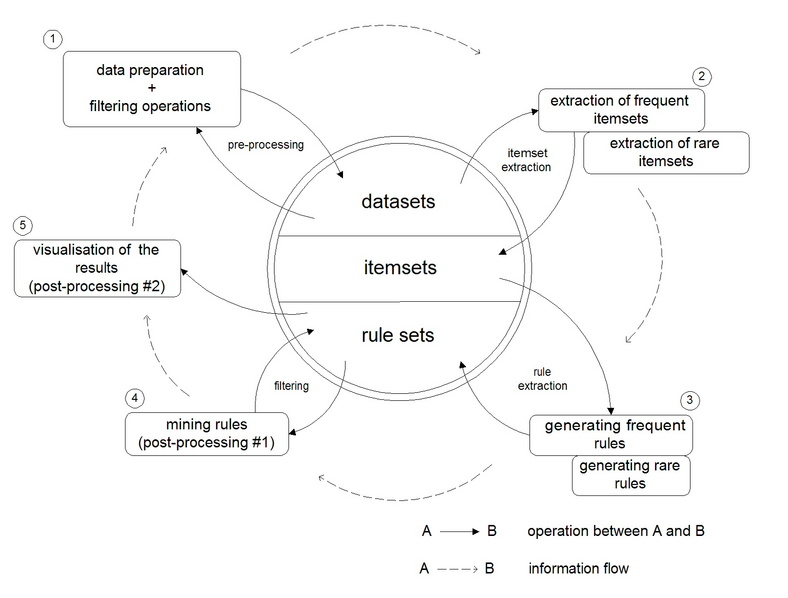
\includegraphics[width=0.95\textwidth]{images/coron-lifecycle.jpg}
	\caption{Ciclo de funcionamiento de la herramientia \eng{Coron System}}
	\label{fig:coron_life_cycle}
\end{figure}

\newpage 

La herramienta \emph{Coron System} provee variados métodos para calcular \abr{FCA} entre ellos se encuentran ``\eng{naive1}'',``\eng{naive2}'', ``\eng{border}'', ``\eng{border2}'' y ``\eng{snow}''. El método que se utilizará para generar la clusterización es el ``\eng{snow}'' dado que esta optimizado mediante los operadores de concepto a encontrar rápidamente el \eng{iceberg lattice} dado un parámetro \eng{minsupp} \cite{snowmethod}\footnote{Para efectos de reducción de costo computacional solo se calculan los \eng{iceberg lattices} y no el \eng{lattice} completo}.

\newpage

\subsection{Extensión de \eng{formal concepts}}
\label{sub:extension_de_formal_concepts}
A partir del \eng{iceberg lattice} obtenido a través del método \eng{snow} con la herramienta \eng{Coron System}, cada concepto es formado por un conjunto de objetos (documentos) y un conjunto de atributos (\eng{tokens}). Sin embargo, debido a la reducción de dimensionalidad realizada, los atributos de cada concepto no superan los 2 o 3 \eng{tokens} máximo. Es por esta razón que es necesario extender los atributos de cada concepto para que cada uno de estos sea representativo de la colección.

La extensión de \eng{formal concepts} se puede apreciar en el siguiente algoritmo:

\begin{algorithm}[h!]
	\caption{Extensión de \eng{Formal Concepts}}
	\label{alg:IntentExtension}
	\begin{algorithmic}[1]
		\Procedure{Formal\textendash Concepts\textendash Extender}{}
		\For{each concept $c \in L$ }
			\State Set $\text{\emph{Tokens}}_c$ as Empty-List
			\For{each document $d \in \text{extent}(c)$ }
			\State Set $W_s$ as words of $d$
				\For{each word $w \in W_s$}
					\If{$w$ is Noun}
						\If{$w \notin \text{Stopwords}$}
							\If{$\text{length}(w) > 3$}
								\State Append $w$ to $\text{\emph{Tokens}}_c$
							\EndIf
						\EndIf
					\EndIf
				\EndFor
			\EndFor
			\State Sort $\text{\emph{Tokens}}_c$ by Frequency
			\State Set $C[\text{intent}] = \text{TOP}(\text{\emph{Tokens}}_c, 50)$
		\EndFor
		\EndProcedure
	\end{algorithmic}
\end{algorithm}

En el algoritmo \ref{alg:IntentExtension} se puede apreciar que por cada \emph{concepto} se obtienen las palabras mas representativas de los titulos, que cumplen con los siguientes criterios:

\begin{enumerate}
	\item Deben ser sustantivos.
	\item El largo de la palabra debe ser mayor a 3.	
	\item No pertenezcan a la lista de \eng{stopwords}.
\end{enumerate}

Por otro lado, a cada concepto se le asignan las $50$ palabras mas relevantes. Esto se debe a que si se incluyen todos los resultados generados cada concepto contará con muchos \eng{tokens} que no son relevantes para el concepto.


\section{Distribución de Tópicos}
\label{sec:distribucion_de_topicos}
Una vez obtenido el \eng{iceberg lattice} correspondiente, junto con el output que genera la herramienta \abr{TMT}, se debe calcular la distribución de tópicos por cada concepto. Esta medida representa ``de qué está hablando el concepto a través de sus documentos''.

Para realizar esto, se utiliza la medida de similitud \eng{Jaccard}

 \begin{definition}{(Similitud de \eng{Jaccard})}
 La similitud de \eng{Jaccard} entre dos conjuntos $A$ y $B$ está dada por:
 \begin{equation*}
	J(A,B) = \frac{\left\vert{A \cap B}\right\vert}{\left\vert{A \cup B}\right\vert}
\end{equation*}
 \end{definition}

 Utilizando la similitud de \eng{Jaccard} dado el conjunto de palabras más relevantes que tiene cada tópico y el conjunto de palabras que conforman el concepto (\eng{intent}) se puede calcular la distribución que tienen los tópicos en cada concepto del \eng{Lattice}

\section{Visualización de Lattice}
\label{sec:visualizacion_de_lattice}
La visualización del lattice requiere que la siguiente información ya se encuentre procesada y disponible:

\begin{enumerate}
	\item \eng{Iceberg Lattice}.
	\item Extensión de \eng{formal concepts}.
	\item Distribución de tópicos por cada concepto.
\end{enumerate}

Para la generación de la visualización del Lattice se partirá de la base que se cuenta con un archivo de grafo en formato \abr{GEXF} donde contendrá la información anterior. Este archivo será la entrada para generar el layout de \eng{lattice} deseado mediante el software Gephi ~\cite{gephi}.


\subsection{Formato \abr{GEXF}}
\label{sub:eng}

\subsubsection{¿Qué es?}
\abr{GEXF} (\eng{Graph Exchange XM Format}) es un lenguaje para describir estructuras de \emph{redes complejas}, con su información y dinámica asociada. Comenzó en el 2007 como un proyecto de \eng{Gephi} por diferentes actores, profundamente envueltos en la problemática de intercambio de grafos. Las especificaciones de \abr{GEXF} son lo suficientemente maduras para declararse extensibles y abiertas, además de adecuado para aplicaciones reales.

\subsubsection{Manifiesto}
Dado que formatos para el intercambio de grafos han existido a lo largo del tiempo, las razones para crear este formato son las siguientes:

\begin{enumerate}
	\item Fuerte base, pero con amplia libertad: la palabra clave del objetivo de crear el formato \abr{GEXF} es el \emph{intercambio}. Esto se hace claro al ver que el formato \abr{GEXF} obliga a respetar la base de la topología de grafos y datos, pero permitir a las personas agregar su propio \eng{namespace} para tener la flexibilidad necesaria para cualquier tipo de negocios.
	\item Solamente la red: el interés común de los autores son las redes complejas, nada más. El objetivo del formato \abr{GEXF} es representar los elementos de una red: nodos, arcos y la data asociada a ello. Manteniendo el formato simple y enfocado en la misma red.
	\item Estructura jerárquica: otros formatos de intercambio de grafos también tienen esta característica. Los nodos pueden contener otros nodos y así sucesivamente. El formato permite la creación de la estructura jerárquica. Esto es fundamental para representar \eng{clustering}.
	\item Utilidad de \abr{XML}: es un lenguaje conocido, tiene capacidad de soporte para utilizar \eng{namespaces} y además existen innumerables motores de base de datos basados en XML.
\end{enumerate}

\subsubsection{Ejemplo}
Este pequeño ejemplo contiene dos nodos y un arco que los relaciona:

\lstset{
  language=XML,
  morekeywords={encoding,
    xs:schema,xs:element,xs:complexType,xs:sequence,xs:attribute,gexf, meta, creator, description, graph, nodes, node, edges, edge, id, label, source, target, xmlns, lastmodifieddate, mode, defaultedgetype}
}
\begin{lstlisting}
<?xml version="1.0" encoding="UTF-8"?>
<gexf xmlns="http://www.gexf.net/1.2draft" version="1.2">
    <meta lastmodifieddate="2009-03-20">
        <creator>Gexf.net</creator>
        <description>A hello world! file</description>
    </meta>
    <graph mode="static" defaultedgetype="directed">
        <nodes>
            <node id="0" label="Hello" />
            <node id="1" label="Word" />
        </nodes>
        <edges>
            <edge id="0" source="0" target="1" />
        </edges>
    </graph>
</gexf>
\end{lstlisting}


\subsection{Gephi - Layout}
\label{sub:gephi_layout}
A partir del archivo en formato \abr{GEXF} se procesará a través de un \eng{layout} personalizado a través del software Gephi.

El \eng{layout} que se creará parte de la base de modelar el grafo en una grilla de alto el número de niveles que tenga \eng{ lattice} y ancho el máximo número de nodos que tenga por cada nivel. para esto, se presenta el código donde se calcula esto:

\lstset{
  basicstyle=\footnotesize\tt,        % the size of the fonts that are used for the code
  breakatwhitespace=false,         % sets if automatic breaks should only happen at whitespace
  breaklines=true,                 % sets automatic line breaking
  captionpos=b,                    % sets the caption-position to bottom
  extendedchars=true,              % lets you use non-ASCII characters; for 8-bits encodings only, does not work with UTF-8
  frame=single,                    % adds a frame around the code
  language=Java,                 % the language of the code
  keywordstyle=\bf,
  showspaces=false,                % show spaces everywhere adding particular underscores; it overrides 'showstringspaces'
  showstringspaces=false,          % underline spaces within strings only
  showtabs=false,                  % show tabs within strings adding particular underscores
  tabsize=2                       % sets default tabsize to 2 spaces
}
\begin{lstlisting}
public class LatticeLayout implements Layout{
    //Architecture
    private final LayoutBuilder builder;
    private GraphModel graphModel;
    //Flags
    private boolean executing = false;
    //Properties
    private int areaSize;
    private float speed;
    private float horizontalRepulsion;
    private int maxLevels;
    private int maxWidth;
    private int getLevelsOfLattice(){
        Graph graph = graphModel.getGraphVisible();
        graph.readLock();
        Node[] nodes = graph.getNodes().toArray();
        int maxLevel = -1;
        int level = -1;
        for(Node n: nodes){
            level = (Integer) n.getAttributes().getValue("Level");
            if(level > maxLevel){
                maxLevel = level;
            }
        }
        graph.readUnlock();
        return maxLevel;
    }
    private int getLatticeWidth(){
        Graph graph = graphModel.getGraphVisible();
        graph.readLock();
        Node[] nodes = graph.getNodes().toArray();
        ConcurrentMap<Integer, Integer> widths = new ConcurrentHashMap<Integer,Integer>();
        int level,maxwidth = -1;
        for(Node n: nodes){
            level = (Integer) n.getAttributes().getValue("Level");
            Integer counter = widths.get(level);
            if(counter == null){
                widths.putIfAbsent(level, 1);
            }
            else{
                widths.replace(level, counter+1);
            }
        }
        for(int i=0; i<this.maxLevels; i++){
            if(widths.get(i)>maxwidth){
                maxwidth = widths.get(i);
            }
        }
        graph.readUnlock();
        return maxwidth;
    }
    private Node[] getNodesByLevel(int level){
        Graph graph = graphModel.getGraphVisible();
        graph.readLock();
        Node[] nodes = graph.getNodes().toArray();
        ArrayList<Node> nodesByLevel = new ArrayList<Node>();
        for(Node n: nodes){
            Integer nodeLevel = (Integer) n.getAttributes().getValue("Level");
            if(nodeLevel == level){
                nodesByLevel.add(n);
            }
        }
        graph.readUnlock();
        Node[] nodesByLevelArray = nodesByLevel.toArray(new Node[nodesByLevel.size()]);
		Arrays.sort(nodesByLevelArray,new Comparator<Node>() {
            @Override
            public int compare(Node o1, Node o2) {
                Number n1 = (Number) o1.getAttributes().getValue("Support");
                Number n2 = (Number) o2.getAttributes().getValue("Support");
                if(n1.doubleValue() < n2.doubleValue()){
                    return 1;
                }
                else if(n1.doubleValue() > n2.doubleValue()){
                    return -1;
                }
                else{
                    return 0;
                }
            }
        });
        return nodesByLevelArray;
    }
    protected void setSizeToTopAndBottom(){
        Graph graph = graphModel.getGraphVisible();
        graph.readLock();
        Node[] nodes = graph.getNodes().toArray();
        for(Node n: nodes){
            if(n.getAttributes().getValue("Type").equals("top") 
                    || n.getAttributes().getValue("Type").equals("bottom")){
                n.getNodeData().setSize(35);
            }
            else{
                n.getNodeData().setSize(15);
            }
        }
        graph.readUnlock();
    }
    @Override
    public void initAlgo() {
        this.executing = true;
        this.maxLevels = this.getLevelsOfLattice();
        this.maxWidth = this.getLatticeWidth();
        this.setSizeToTopAndBottom();
    }
    @Override
    public void goAlgo() {
        Graph graph = graphModel.getGraphVisible();
        graph.readLock();
        int rows = this.maxLevels + 1;
        int cols = this.maxWidth;
        float cell_h = ((float)this.areaSize/rows);
        float cell_w = ((float)this.areaSize/cols) + this.horizontalRepulsion;
        for (int i = 0; i < rows; i++) {
            int j = 0;
            Node[] nodesByLevel = this.getNodesByLevel(i);
            float offset = ((float)(cols - nodesByLevel.length)/2)*((float)cell_w);
            for(Node node: nodesByLevel){
                node.getNodeData().setY(i*cell_h);
                node.getNodeData().setX(offset + j*cell_w);
                j++;
            }
        }
        graph.readUnlock();
    }
    @Override
    public LayoutProperty[] getProperties() {
        List<LayoutProperty> properties = new ArrayList<LayoutProperty>();
        final String LatticeLayout = "Lattice Layout";
        try {
            properties.add(LayoutProperty.createProperty(
                    this, Float.class,
                    "Horizontal Repulsion",
                    LatticeLayout,
                    "The horizontal gap between concepts",
                    "getHorizontalRepulsion","setHorizontalRepulsion"));
            properties.add(LayoutProperty.createProperty(
                    this, Integer.class,
                    "Area size",
                    LatticeLayout,
                    "The area size",
                    "getAreaSize", "setAreaSize"));
            properties.add(LayoutProperty.createProperty(
                    this, Float.class,
                    "Speed",
                    LatticeLayout,
                    "How fast are moving nodes",
                    "getSpeed", "setSpeed"));
        } catch (Exception e) {
            e.printStackTrace();
        }
        return properties.toArray(new LayoutProperty[0]);
    }
}
\end{lstlisting}


Una vez aplicado el \eng{Lattice Layout} sobre el grafo determinado este es posible exportarlo en dos formatos: \abr{GEXF} y \abr{JSON} los cuales son compatibles con la herramienta \eng{Sigma.JS}. Sin embargo, por evaluaciones de rendimiento, se decide exportar el grafo en formato \abr{JSON}.

\subsection{Sigma}
\label{sub:exporter_to_sigma}
Sigma es una libraría de \eng{Javascript} que esta dedicada a dibujar grafos. Hace que sea fácil publicar redes en sitios web donde permite la interacción con el usuario.

Sigma provee muchas características incluidas, como son \eng{renders} en Canvas o WebGL o incluso el soporte de eventos producidos por la interacción con el usuario. Esto permite que la manipulación de grandes redes complejas en páginas web sean fluidas y rápidas para el usuario.

Las características de Sigma.JS permiten una fácil configuración del grafo que se quiere dibujar. Por otro lado, existen extensiones que permiten importar grafos en formato \abr{GEXF} y \abr{JSON} lo cual la hace una librería perfectamente compatible con las posibles salidas del software \eng{Gephi}.

Además, cada nivel tiene sus conceptos ordenados por el valor del soporte de cada concepto de forma decreciente. Esto quiere decir, que el concepto que esté más a la izquierda tendrá un soporte mayor que el de la derecha de su mismo nivel.


%%%%%%%%%%%%%%%%%%%%%%%%%%%%%%%%%%%%%%%%%%%%%%%%%%%%%%%%%%%%%%%%%%%%%%%%
%%%%%%%% 						Resultados 						%%%%%%%%
%%%%%%%%%%%%%%%%%%%%%%%%%%%%%%%%%%%%%%%%%%%%%%%%%%%%%%%%%%%%%%%%%%%%%%%%
\chapter{Resultados}
\section{\eng{Lattices} Generados}
A través de la implementación de este trabajo, se probó con diferentes valores del parámetro \eng{minsupp}, para poder tener una observación tangible de cuán sensible es el \eng{iceberg lattice} a la elección de este parámetro.

Los resultados se presentan a continuación:

\begin{table}[h!]
\centering
\caption{Diferentes \eng{iceberg lattices} con diferentes parámetros \eng{minsupp}}
\label{tbl:minsupp_sensibility_table}
\begin{tabular}{|l|l|l|l|}
\hline
\multicolumn{1}{|c|}{{\bf \begin{tabular}[c]{@{}c@{}}Minimal Support\\ Relative\end{tabular}}} & \multicolumn{1}{c|}{{\bf \begin{tabular}[c]{@{}c@{}}Minimal Support\\ Absolute\end{tabular}}} & \multicolumn{1}{c|}{{\bf \#Concepts}} & \multicolumn{1}{c|}{{\bf \#Levels}} \\ \hline
					$0.0005$ 	& 	$15$ 		& 	$221574$ 	& 	$9$ 	\\ \hline
					$0.0009$ 	& 	$26$ 		& 	$132517$ 	& 	$7$ 	\\ \hline
					$0.001$ 	& 	$29$ 		& 	$119475$ 	& 	$7$ 	\\ \hline
					$0.005$ 	& 	$147$ 		& 	$18903$ 	& 	$6$ 	\\ \hline
					$0.009$ 	& 	$265$ 		& 	$8123$ 		& 	$6$ 	\\ \hline
					$0.01$ 		& 	$294$ 		& 	$6945$ 		& 	$5$ 	\\ \hline
					$0.05$ 		& 	$1472$ 		& 	$1098$ 		& 	$4$ 	\\ \hline
\rowcolor{gray!25}\color{blue} 	$0.09$ 		& 	$2650$ 		& 	$833$ 		& 	$4$ 	\\ \hline
\rowcolor{gray!25}\color{blue} 	$0.5$ 		& 	$14721$ 	& 	$159$ 		& 	$2$ 	\\ \hline
					$1$ 		& 	$29443$ 	& 	$38$ 		& 	$2$ 	\\ \hline
					$2$ 		& 	$58886$ 	& 	$0$ 		& 	$0$ 	\\ \hline
\end{tabular}
\end{table}
\newpage
La tabla anterior, genera la siguiente gráfica:

\begin{figure}[h!]
	\centering
	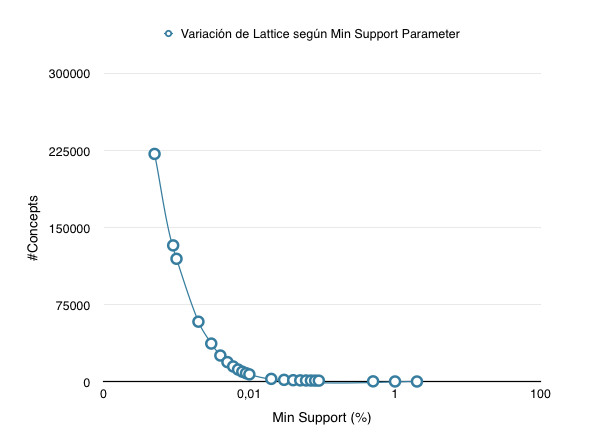
\includegraphics[width=0.90\textwidth]{images/minsupp_sensibility.png}
	\caption{Sensibilidad del parámetro \eng{Minimal Support} correspondiente a la información de la Tabla~\ref{tbl:minsupp_sensibility_table}}
	\label{fig:minsupp_sensibility}
\end{figure} 

Donde se puede ver que la cantidad de conceptos decrece exponencialmente. Esto se debe a que la información utilizada para generar el lattice, particularmente el \eng{Formal Context} es una matriz muy dispersa dada la misma naturaleza de los datos. Pocos \eng{tokens} en comparación con la cantidad de documentos.

\section{\eng{Lattice} Navegable}
Es la página principal del sitio web, en donde se presenta el \eng{Iceberg Lattice} para diferentes soportes: $0.5$ y $0.09$.

\begin{figure}[h!]
	\centering
	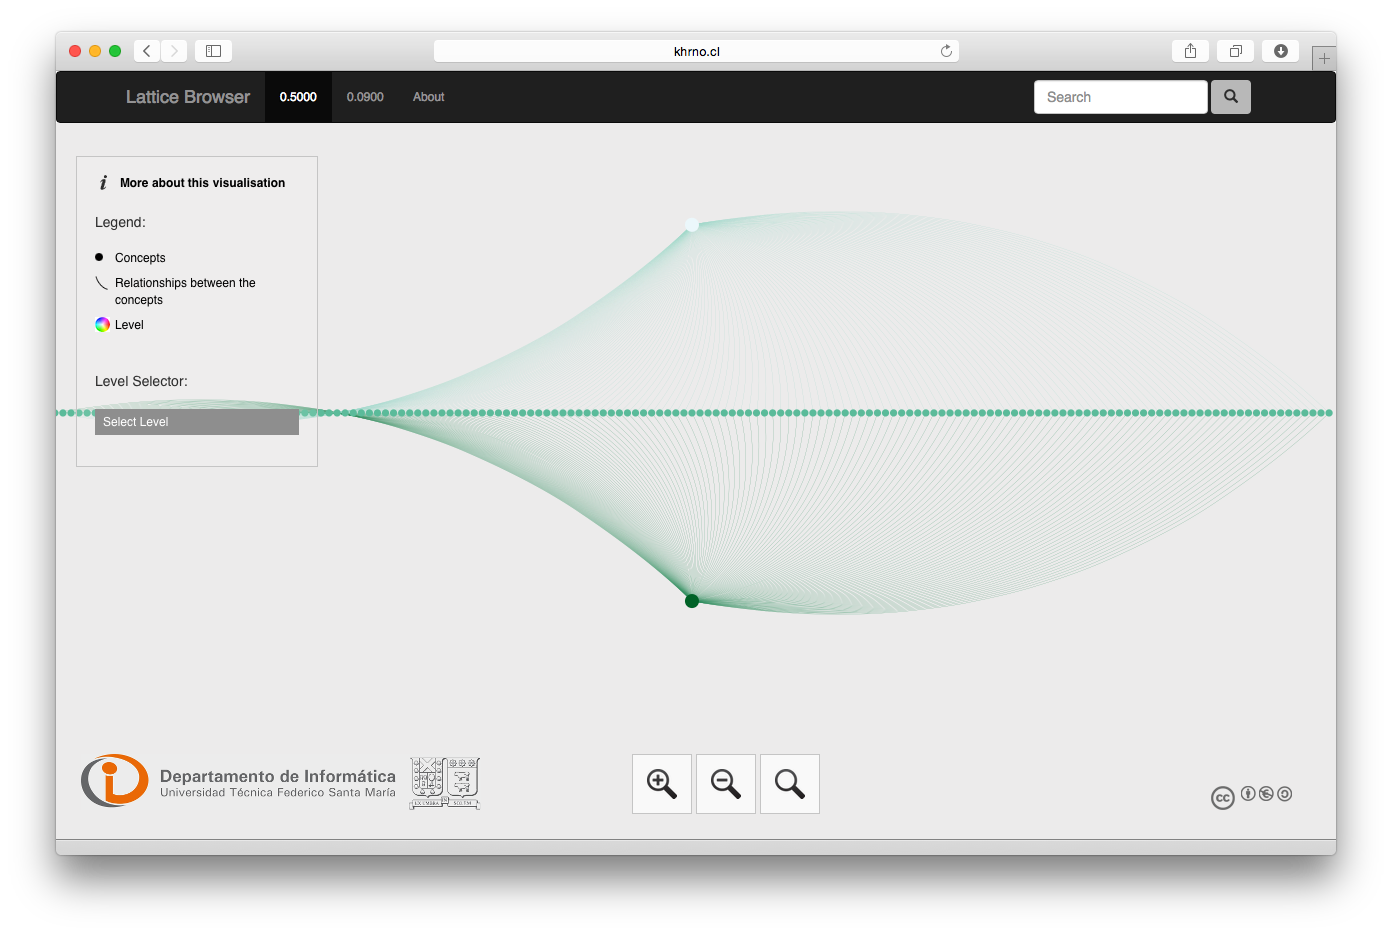
\includegraphics[width=0.90\textwidth]{images/results_1.png}
	\caption{Página principal de la visualización del \eng{Lattice}.}
	\label{fig:results_1}
\end{figure} 

Aquí es donde se encuentra la mayor interacción con el usuario, ya que utilizando las herramientas que se detallan en la figura \ref{fig:results_2} este puede cambiar la visualización al \eng{Iceberg Lattice} de soporte $0.5$ o bien a la visualización del \eng{Iceberg Lattice} con soporte de $0.09$. Por otro lado, el usuario puede buscar los conceptos que contengan los \eng{top-terms} mas relevantes dado por su frecuencia.

\begin{figure}[h!]
	\centering
	
\includegraphics[width=1\textwidth]{images/results_2.png}
	\caption{Cambio de soporte y buscador\eng{Lattice}}
	\label{fig:results_2}
\end{figure}

Por otra parte, como se muestra en la figura \ref{fig:results_3} se puede seleccionar todos los conceptos de un determinado nivel determinado, al hacer esto, se carga un panel al lado derecho para que el usuario seleccione que concepto desea ver más en detalle.

\begin{figure}[h!]
	\centering
	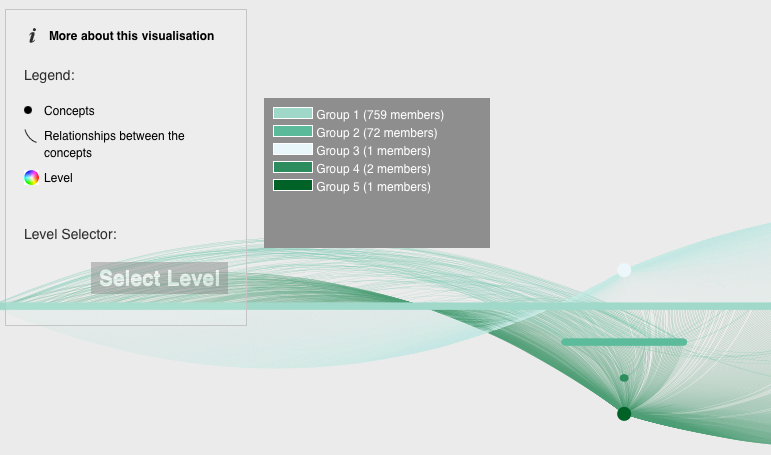
\includegraphics[width=1\textwidth]{images/results_3.png}
	\caption{Selección de conceptos del mismo nivel}
	\label{fig:results_3}
\end{figure}

Asimismo, cuando el usuario selecciona, o directamente del grafo o a través de la búsqueda o por medio del filtrado por nivel, un concepto específico se abre un panel de información detallada de este concepto que contiene la siguiente información. Tal como se muestra en la figura \ref{fig:results_4}.

 \begin{figure}[h!]
	\centering
	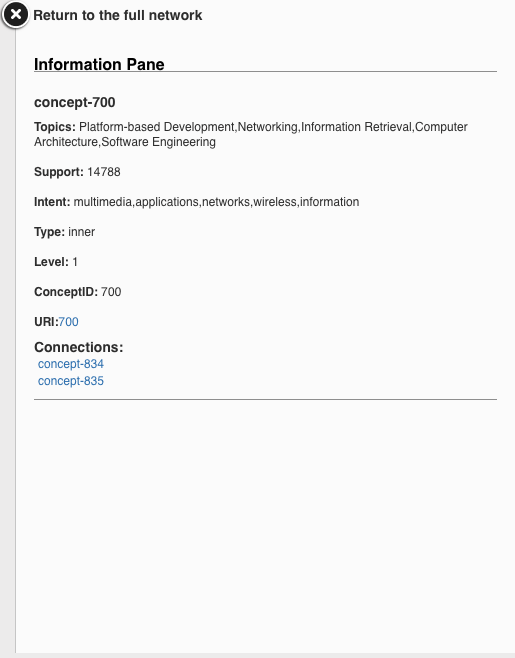
\includegraphics[width=0.8\textwidth]{images/results_4.png}
	\caption{Panel de información de un concepto}
	\label{fig:results_4}
\end{figure}

\begin{itemize}
	\item Identificador del concepto.
	\item Principales tópicos (con mayor similitud al concepto).
	\item Principales términos que conforman el concepto (basados en la frecuencia de ocurrencia).
	\item El soporte absoluto.
	\item El tipo de nodo que es, pueden existir tres tipos de nodos por la naturaleza de los \eng{Lattices} y estos son: ``\eng{inner}'', ``\eng{bottom}'', ``\eng{top}''.
	\item El nivel donde está ubicado el concepto en el \eng{Lattice}.
	\item La URI para navegar a la pantalla de detalles del concepto.
	\item Las conexiones que tiene el concepto en el \eng{Lattice}.
\end{itemize}

De este mismo modo, existen los botones de navegación dentro de la misma red. Como se muestran en la figura \ref{fig:results_5}.
\begin{figure}[h!]
	\centering
	
\includegraphics[width=0.3\textwidth]{images/results_5.png}
	\caption{Botones de navegación globales}
	\label{fig:results_5}
\end{figure}


\section{Detalles del Concepto}
La página de los detalles del concepto permite ver como se conforma el mismo, además de la posición que toma dentro del \eng{Lattice} que lo contiene. Por otro lado, está página permite moverse a través del vecindario del concepto que estoy viendo, es decir, ir al concepto de la derecha, izquierda, arriba o abajo.

\begin{figure}[h!]
	\centering
	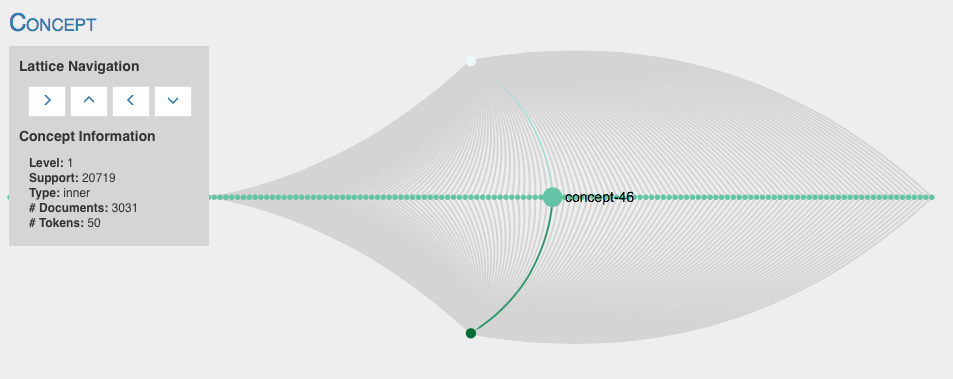
\includegraphics[width=1\textwidth]{images/results_6.png}
	\caption{Navegación detallada dentro del vecindario del concepto}
	\label{fig:results_6}
\end{figure}

La figura \ref{fig:results_6} representa la ubicación del concepto que se está observando junto con algunos atributos transversales en todos los conceptos como son: nivel, soporte, tipo de concepto, número de documentos, número de \eng{tokens}. Además se puede apreciar los botones de navegación del vecindario del concepto. Con estos botones, el usuario puede ir hacia el concepto que está ubicado a la derecha, izquierda, arriba o abajo.

 \begin{figure}[h!]
	\centering
	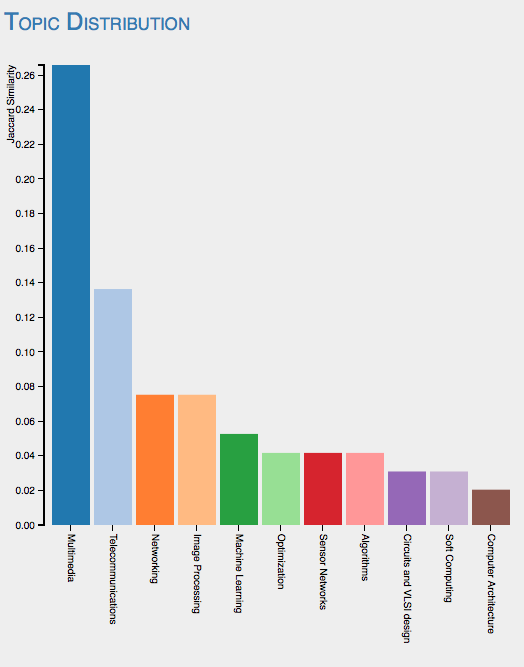
\includegraphics[width=0.8\textwidth]{images/results_7.png}
	\caption{Distribución de tópicos del concepto}
	\label{fig:results_7}
\end{figure}

En la figura \ref{fig:results_7} se puede apreciar un gráfico que representa la distribución de tópicos que conforman el concepto. En este caso particular, se puede apreciar claramente que el concepto mayoritariamente es sobre el tópico ``Multimedia''.

 \begin{figure}[h!]
	\centering
	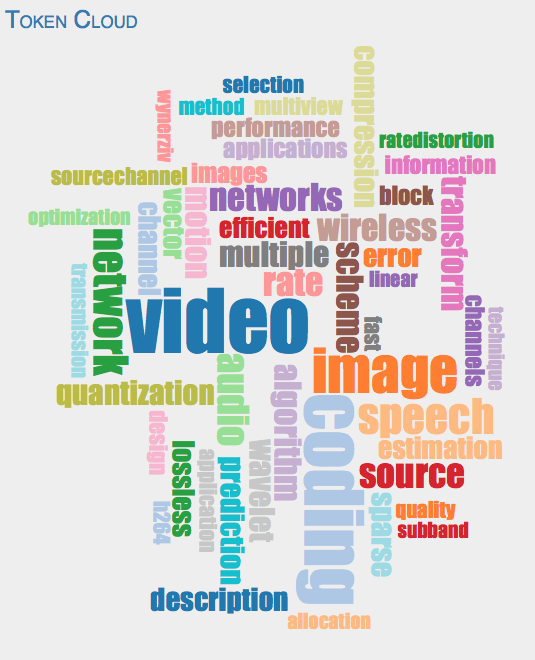
\includegraphics[width=0.8\textwidth]{images/results_8.png}
	\caption{\eng{Token Cloud} que forman el concepto}
	\label{fig:results_8}
\end{figure}

Asimismo, en la figura \ref{fig:results_8} se puede ver una nube de \eng{tokens} que son relevantes para el concepto. La definición de relevancia es determinado por la frecuencia de ocurrencias que tiene las palabras dentro de los mismos documentos que lo forman.

\newpage

 \begin{figure}[h!]
	\centering
	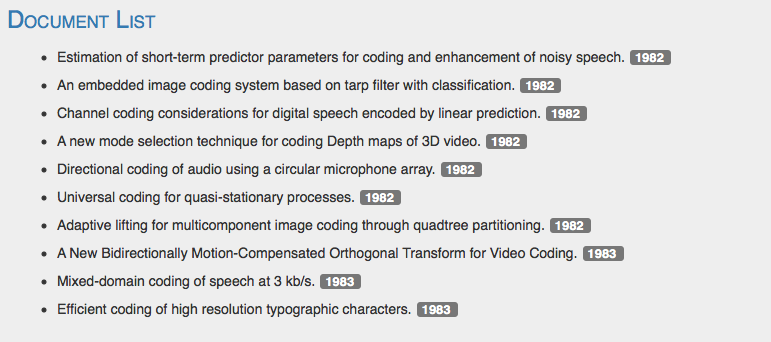
\includegraphics[width=0.9\textwidth]{images/results_9.png}
	\caption{Lista de documentos - objetos - que forman el concepto}
	\label{fig:results_9}
\end{figure}

Por otro lado, la sección ilustrada por la figura \ref{fig:results_9} indica la colección de documentos presentes en el concepto. Dado que en la mayoría de los conceptos la cantidad de documentos que lo conforman es muy alta, se decidió paginar estos resultados.

%%%%%%%%%%%%%%%%%%%%%%%%%%%%%%%%%%%%%%%%%%%%%%%%%%%%%%%%%%%%%%%%%%%%%%%%
%%%%%%%% 					Conclusiones 						%%%%%%%%
%%%%%%%%%%%%%%%%%%%%%%%%%%%%%%%%%%%%%%%%%%%%%%%%%%%%%%%%%%%%%%%%%%%%%%%%
\chapter{Conclusiones}
Durante el desarrollo del presente trabajo fue posible generar una clusterización jerárquica suave de una gran colección de documentos científicos, utilizando dos técnicas separadamente para enfrentar el gran problema de la dimensionalidad de los datos. De esta forma, se logró comprobar que existen modelos matemáticos que por si solos o son lo suficientemente capaces de manejar grandes cantidades de información, como es el caso de \abr{FCA}, sin embargo, al utilizarlos junto a otros modelos estadísticos, particularmente \abr{LDA}, forman una gran dupla que permiten resolver - al menos de modo parcial - uno de los principales problemas que existen en el día de hoy: una inconmensurable cantidad de información y una alta aceleración en la producción de la misma.

Por otro lado, si se observa cuidadosamente los resultados obtenidos, se puede comprobar que si existe una relación adecuada entre los resultados de la técnica \abr{LDA} y los resultados de la técnica \abr{FCA}. Como por ejemplo, si se toma el caso particular el concepto que tiene id $46$ (Figura \ref{fig:conclusiones_1}), se puede observar que los \eng{tokens} más relevantes del concepto son: ``\eng{Video}'', ``\eng{Coding}'', ``\eng{image}'', los cuales tiene mucha relación como descriptores de los tópicos ``\eng{Multimedia}'' y ``\eng{Telecommunications}'' que corresponden a ser los que mayor relación tienen con el concepto.

 \begin{figure}[h!]
	\centering
	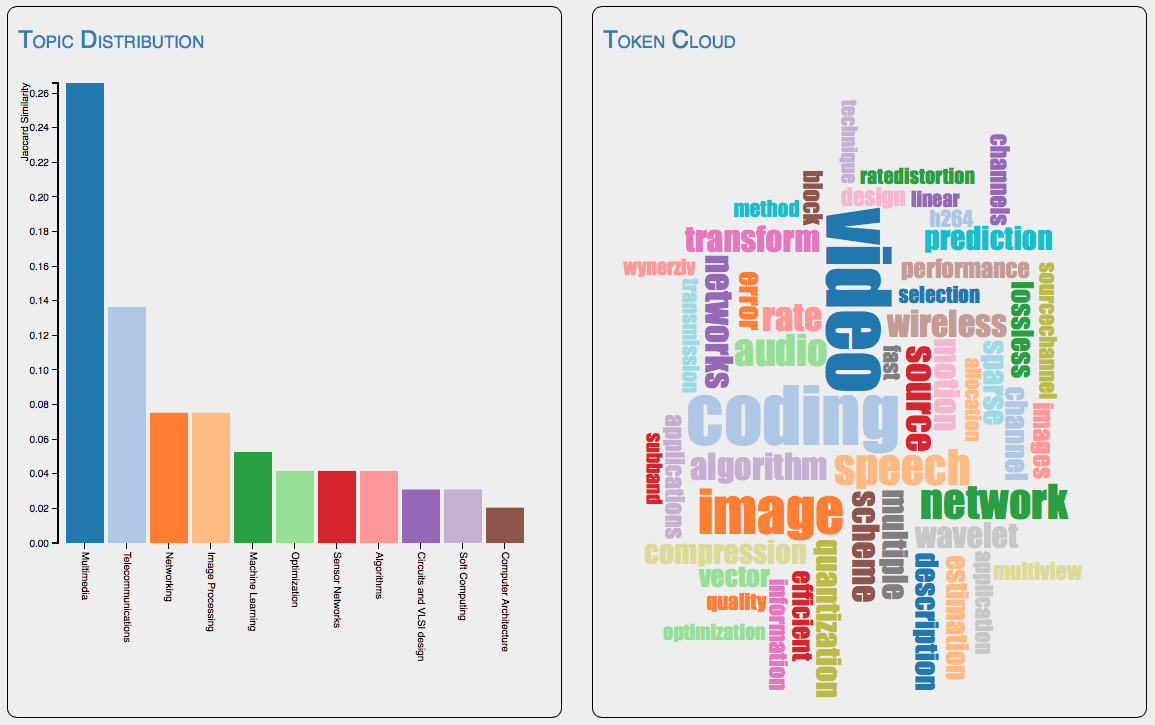
\includegraphics[width=1\textwidth]{images/conclusiones_1.png}
	\caption{Relación entre resultados de \abr{FCA} y \abr{LDA}}
	\label{fig:conclusiones_1}
\end{figure}

Asimismo, con el objetivo de visualizar los resultados realizados por este trabajo, se logro comprobar que existen herramientas (\eng{Gephi} y \eng{SigmaJS}) que permite facilitar la visualización de grandes colecciones de redes complejas. Es más, las herramientas utilizadas para la generación del navegador del \eng{Lattice} componen tres grandes características que las hacen una gran elección para visualizar grandes redes complejas:

\begin{itemize}
	\item Flexibilidad: entrega al usuario la capacidad de utilizarlas de acuerdo a sus necesidades sin mayores problemas.
	\item Robustas: permiten trabajar con una gran cantidad de información con la seguridad que no fallarán. 
   	\item Pertenecen al mundo del \eng{open source}: permite que las personas interesadas puedan extenderlas, modificarlas utilizarlas sin pagar licencias de altos costos.
   \end{itemize}   

%%%%%%%%%%%%%%%%%%%%%%%%%%%%%%%%%%%%%%%%%%%%%%%%%%%%%%%%%%%%%%%%%%%%%%%%
%%%%%%%% 					Trabajo Futuro 						%%%%%%%%
%%%%%%%%%%%%%%%%%%%%%%%%%%%%%%%%%%%%%%%%%%%%%%%%%%%%%%%%%%%%%%%%%%%%%%%%
\chapter{Trabajo Futuro}
\section{Componente Social}
En este trabajo, para una determinada colección de artículos científicos (\abr{DBLP}) se generó una clusterización basada en los títulos y las palabras claves que lo componen. Como trabajo futuro se plantea agregar una componente social a dicha colección a través de las redes de colaboración entre autores de los trabajos. Esto permitirá generar una red social de autores, en la cual se plantea detectar las comunidades científicas y una vez detectadas, observar como se comporta el conocimiento de dicha comunidad, es decir, responder a la pregunta ¿Qué ha estado trabajando la comunidad de investigadores relacionada por ejemplo, con el cáncer?.

\section{Descriptores de cada objeto}
Como futuro trabajo se plantea cambiar extender o cambiar la colección para que se incluyan los \eng{abstracts} de cada documento, lo cual permitiría una clasificación a través de la técnica {FCA} más suavizada ya que el \eng{Formal Context} tendría una mayor densidad en proporción a la cantidad de palabras que componen un título comparado con la cantidad de palabras que componen un \eng{abstract}.


%%%%%%%%%%%%%%%%%%%%%%%%%%%%%%%%%%%%%%%%%%%%%%%%%%%%%%%%%%%%%%%%%%%%%%%%
%%%%%%%% 					Bibliografia 						%%%%%%%%
%%%%%%%%%%%%%%%%%%%%%%%%%%%%%%%%%%%%%%%%%%%%%%%%%%%%%%%%%%%%%%%%%%%%%%%%

\begingroup
\titleformat{\chapter}[display]
  {\Large\scshape}
  {\thechapter}
  {-2em}
  {}

\bibliographystyle{plain} % Se configura el estilo de las referencias puede ser: [plain, abbrv, apalike, ...]
\bibliography{memoria} % Se llama al archivo memoria.bib que contiene las referencias
\endgroup

\end{document}